%!TEX root = ../DSGEnotes.tex
\chapter{最大似然估计}
\label{sec:mle-model}

\epigraph{The maximum-likelihood procedure in any problem is what you are most likely to do if you don’t know any statistics.}{\textit{Harrison H. Barrett \\ Foundations of Image Science}}

\section{线性模型}
\label{sec:linear-model}

设一组含有$n$个观察数据的随机变量$\left\{ y_{i} \right\}, \, i = 1,\ldots,n$。假定其中每个观察符合正态分布$y_{i} \sim \mathcal{N} \left( \mu_{i}, \sigma^{2} \right)$。由设定可见,对于$i,j \in [1,n], \, i \neq j$,均值也许不同,但方差相同。

正态分布(normal distribution)\index{normal distribution! \dotfill 正态分布}又称高斯分布(Gaussian distribution)\index{Gaussian distribution \dotfill 高斯分布},如$y_{i}$的概率密度方程(probability density function, PDF)\index{probability density function (PDF) \dotfill 概率密度方程} $f\left( y_{i} \right)$定义为
\begin{equation}
  \label{eq:mle-pdf-def}
  f \left( y_{i} \right) = \frac{1}{\sqrt{2 \pi \sigma^{2}}}
  \exp \left[
  - \frac{1}{2} \frac{
  \left( y_{i} - \mu_{i} \right)^{2}
  }{
  \sigma^{2}
  }
   \right],
\end{equation}
均值为$0$方差为$1$的高斯分布,见图\ref{fig:mle-pdf}所示。

\begin{lstlisting}[language=R]
# 正态分布的概率密度方程(均值=0,方差=1)
x <- seq(-4,4,length=100)
hx <- dnorm(x)
plot(hx ~ x, type="l", lty = 1, col="blue",
     xlab="y", ylab="Density",
     main = "Probability Density Function (normal distribution)")
\end{lstlisting}

\begin{figure}[htbp]
  \caption{正态分布的概率密度方程}
  \centering
  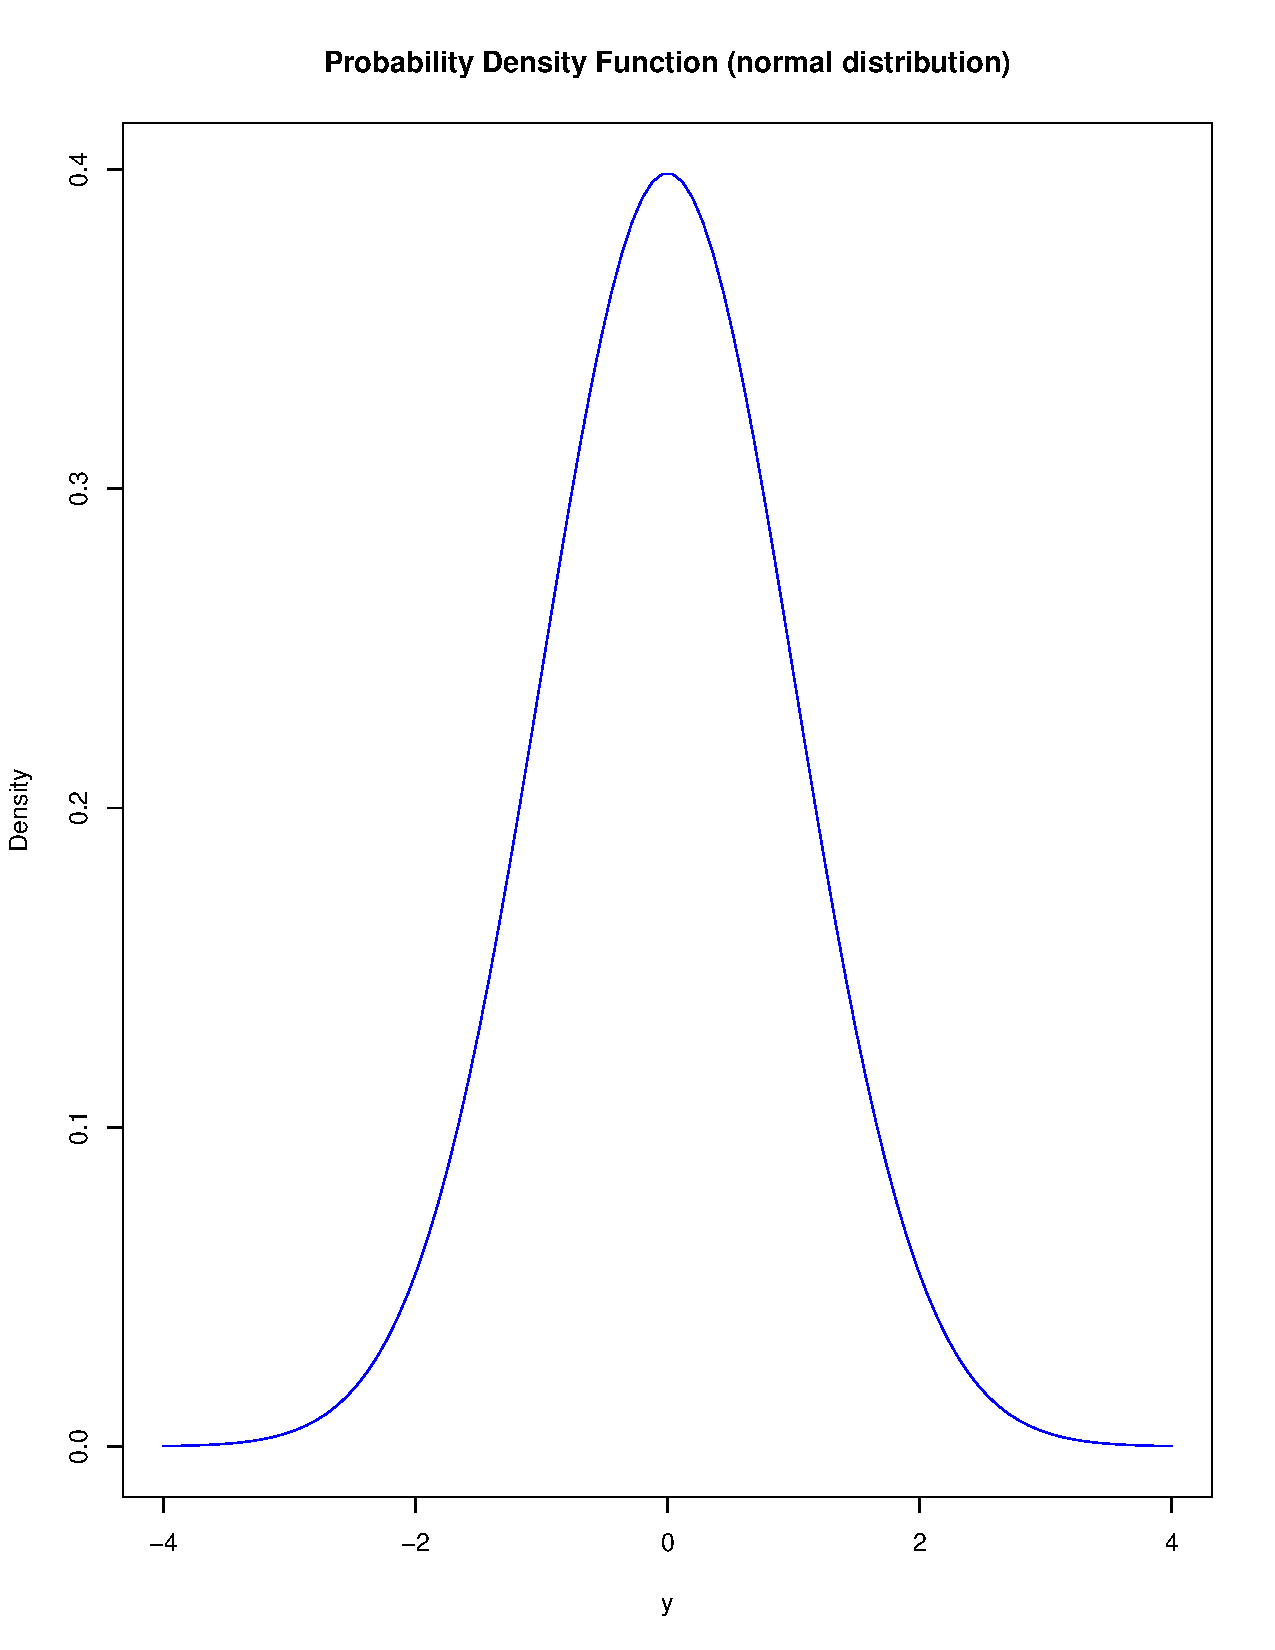
\includegraphics[width=8cm]{./Figures/20180421-pdf-function}
  \label{fig:mle-pdf}
%
%  \small{Source: PBOC.}
\end{figure}

现在引入额外的假定,对于全部$i, j \in [0,n], \, i \neq j$,设观测数据$y_{i}$和$y_{j}$相互独(mutually independent),即$\cov \left( y_{i}, y_{j} \right) = 0$。这使得我们能够计算观测数据集中全部数据的联合分布(joint distribution),即$\prod_{i=1}^{n} f \left( y_{i} \right)$,进而勾勒出似然方程,用于进一步的估计和检测。

把$\left\{y_{i}\right\}_{i=1}^{n}$表示为一个$(n \times 1)$的列向量$Y$,对应均值$E Y = \mu$,方差协方差矩阵$\var(Y) = \sigma^{2} I$,其中$I$是单位矩阵。列向量$\mu = \left\{ \mu_{i} \right\}_{i=1}^{n}$。
由于$n$个观测变量$y_{i}$彼此不相关且方差相同,$\var(Y)$满足以下特征:对角元素全是$\sigma^{2}$,非对角元素全是$0$。进而$Y$呈多元正态分布(multivariate normal distribution)\index{normal distribution!multivariate \dotfill 多元正态分布}
\begin{equation}
  \label{eq:multivariate-normal-distribution}
  Y \sim \mathcal{N}_{n} \left( \mu, \sigma^{2} I \right).
\end{equation}

来看\eqref{eq:multivariate-normal-distribution}的模型。假定$Y = y_{1}, y_{2}, \ldots, y_{n}$与某组预测变量$X = x_{1}, x_{2}, \ldots, x_{n}$有关,进一步说,第$i$个观测变量$y_{i}$的期望值$\mu_{i}$,与$x_{i1}, x_{i2}, \ldots, x_{ip}$有关,呈线性关系,满足
\begin{equation}
  \label{eq:mle-linear-relationship-yx-np}
  \mu_{i} = \beta_{1} x_{i1} + \beta_{2} x_{i2} + \ldots + \beta_{p} x_{ip} \Longleftrightarrow \mu_{i} = x_{i}^{\top} \beta,
\end{equation}
其中$x_{i}^{\top}$是由$p$个预测变量$x_{i1}, x_{i2}, \ldots ,x_{ip}$组成的行向量。待求解的未知系数$\beta = \beta_{1}, \ldots, \beta_{p}$称回归系数。将全部$n$个\eqref{eq:mle-linear-relationship-yx-np}加总可得
\begin{equation}
  \label{eq:mle-linear-relationship-mu-x-beta}
  \underset{\left( n \times 1 \right)}{\mu} =
  \underset{\left( n \times p \right)}{X}
  \underset{\left( p \times 1 \right)}{\beta},
\end{equation}
我们常将解释变量的矩阵$X$称为模型矩阵(model matrix)\index{model matrix \dotfill 模型矩阵}或设计矩阵(design matrix)\index{design matrix \dotfill 设计矩阵}。对应地,$X \beta$称线性预测子(linear predictor)。

最简单的线性模型可以假定每个观测数据的期望值都相同$\mu_{i} = \mu \, \forall \, i$,称零模型(null model)\index{null model \dotfill 零模型}。另一个极端是$\mu_{i} \neq \mu_{j} \, \forall \, i \neq j$,称饱和模型(saturated model)\index{saturated model \dotfill 饱和模型},此时观测数据量$n$越大,待估计的线性系数$\beta$数量就越多($p \times n$)。

零模型和饱和模型是两个极端。现实应用中常取折中,致力于分析导致线性预测子$X \beta$产生结构差异的系统性原因,进而分析观测数据$y$和均值$\mu$之间的非结构性差异(或称随机差异),用误差项来表示。

\section{参数估计}
\label{sec:mle-parameter-estimation}
来看模型$\mu_{i} = x_{i}^{\top} \beta$。问题:如何估计参数$\beta, \sigma^{2}$?

\subsection{回归系数的估计}
\label{sec:mle-estimation-beta}
我们的求解思路是,建立似然方程(likelihood function, LHF)\index{likelihood function (LHF)\dotfill 似然方程},选取使(对数)似然方程最大化的参数值。如果观测数据之间互相独立,那么LHF是一组正态PDF \eqref{eq:mle-pdf-def}的乘积
\begin{equation}
  \label{eq:mle-lhf-pdf-product}
  \log L \left( \beta, \sigma^{2} \right) = - \frac{n}{2} \log \left( 2 \pi \sigma^{2} \right) - \frac{1}{2} \sum_{i=1}^{n}
  \frac{
  \left( y_{i} - \mu_{i} \right)
  }{
  \sigma^{2}
  },
\end{equation}
$\mu_{i}$如\eqref{eq:mle-linear-relationship-yx-np}所定义。RHS中可定义残差平方和(residual sum of squares, RSS)\index{residual sum of squares (RSS) \dotfill 残差平方和}
\begin{equation}
  \label{eq:mle-rss-def}
  RSS (\beta) = \sum_{i=1}^{n} \left( y_{i} - \mu_{i} \right)^{2}
  = \left( y - X \beta \right)^{\top} \left( y - X \beta \right).
\end{equation}

不难看出,在给定$\sigma^{2}$值不变的情况下,最佳系数$\hat{\beta}$的选取符合
\begin{equation}
  \label{eq:mle-lhf-argmax-beta}
  \hat{\beta} =\underset{\beta}{\argmax} \log L \left( \beta, \sigma^{2} \right)
  = \underset{\beta}{\argmin} \frac{\rss(\beta)}{\sigma^{2}},
\end{equation}
也即,我们的目标是选取合适的$\beta = \hat{\beta}$,使对应的模拟值$\mu_{i}$尽可能接近实际观测值$y_{i}$。

求解$\argmin \rss (\beta)$等价于求解$\rss \left( \hat{\beta} \right) =0$,即
\begin{equation*}
  y - X \hat{\beta} = 0 \quad \Rightarrow y = X \hat{\beta} \quad \Rightarrow X^{\top} y = X^{\top} X \hat{\beta}
\end{equation*}
如果模型矩阵$X$列满秩,那么$X^{\top} X$也是满秩的,因而$X^{\top} X$可逆。由此可得线性系数$\hat{\beta}$的OLS估计式(同时也是MLE估计式)
\begin{equation}
  \label{eq:mle-argmin-beta-hat-estimation}
  \hat{\beta} = \left( X^{\top} X \right) X^{\top} y.
\end{equation}
我们将这个方程称为正规方程(normal equation)\index{normal equation \dotfill 正规方程}。

反之,如果$X$不是列满秩的,可以计算$\left( X^{\top} X \right)^{\dagger}$,称为伪逆矩阵(第\ref{sec:simple-pseudo}节)。但比起这种相对复杂的计算来,还是直接删除$X$中的冗余列更加方便。当前大多数主流统计软件都足够只能,可以自动识别并删除冗余列。

求解正规方程\eqref{eq:mle-argmin-beta-hat-estimation}需要借助数值方法。数值方法有多种,常见的如
\begin{itemize}
  \item 从$\left( X^{\top} X \right)$入手,方法如高斯消元法(第\ref{sec:numlin-gaussian-elimination}节)、Cholesky分解(第\ref{sec:numlin-factorization-cholesky}节)等。
  \item 对模型矩阵$X$做因子分解,如
  \begin{itemize}
    \item Householder reflections
    \item Givens rotations
    \item Gram-Schmidt正交(第\ref{sec:orthogonality-polynomials}节),等
  \end{itemize}
\end{itemize}
结合大多数主流数值计算软件,可以执行上述数值运算。

基于\eqref{eq:mle-lhf-argmax-beta},利用最小化RSS方法测得的系数$\hat{\beta}$,是一个不依赖于$\sigma^{2}$的值——方差值是事先给定的。因此我们称$\hat{\beta}$为最大似然法的全局最大解(global maximum)。

对于零模型的情况:$X$是一组$1$构成的向量;$\left( X^{\top} X \right) = n$和$X^{\top} y = \sum_{i=1}^{n} y_{i}$是两个标量;$\hat{\beta} = \bar{y}$是样本的均值。这就是说,计算出的样本均值,可堪称是在线性模型中做最大似然估计的一个最简单的例子。

关于MLE $\hat{\beta}$,有以下几个有趣的性质。

\begin{enumerate}
\item BLUE
\begin{enumerate}
  \item 如果模型设定正确,即从(弱的)意义上说,给定$x_{i}$的情况下,观测$y_{i}$的期望值$\mu_{i}$就等于$x_{i}^{\top} \beta$,此时的OLS估计$\hat{\beta}$是个无偏估计(unbiased estimator),OLS 估计$\hat{\beta}$的期望值就等于真实参数值$\beta$
\begin{equation}
  \label{eq:mle-hat-beta-unbiased}
  E \hat{\beta} = \beta.
\end{equation}
  \item 如果观测数据之间彼此不相关$\cov \left(y_{i}, y_{j} \right) = 0, \, \forall \, i \neq j$,并且同方差$\sigma_{i}^{2} = \sigma_{j}^{2}= \sigma^{2}$。那么,一方面根据\eqref{eq:mle-rss-def}-\eqref{eq:mle-lhf-argmax-beta},$\hat{\beta}$是一个关于$y$的线性方程,另一方面根据假定,观测数据集合$Y$的方差协方差矩阵$\var(Y) = \sigma^{2} I$,那么OLS估计$\hat{\beta}$的方差协方差矩阵为
  \begin{equation}
    \label{eq:mle-hat-beta-varcov}
    \var \left( \hat{\beta} \right) = \left( X^{\top} X \right)^{-1} \sigma^{2},
  \end{equation}
  因此,基于观测数据,构建线性方程模型所做的全部无偏OLS估计$\left\{\beta\right\}$中,MLE估计$\hat{\beta}$是最佳线性无偏估计(best linear unbiased estimator, BLUE)\index{best linear unbiased estimator (BLUE) \dotfill 最佳线性无偏估计}。对于某一给定的观测样本,由于再没有其他无偏估计的方差会低于$\var \left( \hat{\beta} \right)$,我们称OLS估计$\hat{\beta}$是有效估计(efficient estomator)\index{efficient estimator \dotfill 有效估计}。
\end{enumerate}

\item OLS估计$\hat{\beta}$在大样本观测集合中的抽样分布,接近于多元正态分布,其均值和方差如\eqref{eq:multivariate-normal-distribution}所定义,满足
\begin{equation*}
  \hat{\beta} \sim \mathcal{N}_{p} \left( \beta, \left(X^{\top}, X \right)^{-1} \sigma^{2} \right).
\end{equation*}

\item 将前两个性质代入零模型,可见样本均值$\bar{y}$是对$\mu$的无偏估计;$\bar{y}$的方差为$\frac{\sigma^{2}}{n}$,在大样本下近似正态分布。

\item 前三条性质的生成,依赖于对观测数据的均值、方差协方差的最高到二阶矩条件的假设,包括
\begin{equation*}
  E Y = X \beta, \quad \var \left( Y \right) = \sigma^{2} I.
\end{equation*}

\item 基于观测数据的联合正态分布假定,所测得的OLS估计$\hat{\beta}$也是MLE。如果$Y \sim \mathcal{N}_{p} \left( X \beta, \sigma^{2} I \right)$,那么$\hat{\beta}$的样本分布恰好也是多元正态分布,对应的、方差也是
\begin{equation*}
  \hat{\beta} \sim \mathcal{N}_{p} \left( \beta, \left(X^{\top}, X \right)^{-1} \sigma^{2} \right).
\end{equation*}.
\end{enumerate}

需要指出的是,上属性质虽然重要,但不应被过分夸大:只有在小样本数据的统计推断中,才需要假定观测数据是正态分布的。而真正重要的假设其实是观测数据之间彼此不相关,同方差:这些对于大样本数据下的统计推断至关重要。

\subsection{方差的估计}
\label{sec:mle-estimation-variance}
将求得的OLS估计$\hat{\beta}$ \eqref{eq:mle-argmin-beta-hat-estimation}代回log LHF \eqref{eq:mle-lhf-pdf-product},可得一个关于方差$\sigma^{2}$的最大(对数)似然方程,又称描述似然方程(profile likelihood function)\index{profile likelihood function \dotfill 描述似然方程}
\begin{equation}
  \label{eq:mle-estimation-variance-plhe}
  \log L \left( \sigma^{2} \right)
  = - \frac{n}{2} \log \left( 2 \pi \sigma^{2} \right)
  - \frac{1}{2} \frac{
  \rss \left( \hat{\beta} \right)
  }{\sigma^{2}}.
\end{equation}

类似地,$\hat{\sigma}^{2} = \underset{\sigma^{2}}{\argmax} \, \log L \left( \sigma^{2} \right)$,等价于求解$\frac{\partial \log L \left( \sigma^{2} \right)}{\partial \sigma^{2}} = 0 $,求得的值为方差的MLE
\begin{equation*}
  \hat{\sigma}^{2} = \frac{\rss \left( \hat{\beta} \right)}{n},
\end{equation*}
需要指出的是,$\hat{\sigma}^{2}$是有偏估计;我们可以将分母用$n-p$代替$n$来变为无偏估计(类似于在估计方差时用$n-1$代替$n$)。

在零模型中,方差$\sigma^{2}$的估计是样本方差:这是由于$\hat{\beta} = \bar{y}, \, \rss = \sum_{i=1}^{n} \left( y_{i} - \bar{y} \right)$。在正态分布的假定条件下,比值$\left( \frac{\rss }{\sigma^{2}}\right)$呈$\chi^{2}$分布(DoF n-p),并且与线性系数估计值$\hat{\beta}$无关。

小提示:使用$\chi^{2}$分布作为LHF来估计$\sigma^{2}$,比起使用高斯分步来同时估计$\beta, \sigma^{2}$来,会得到无偏估计。

\section{假设检验}
\label{sec:mle-hypothesis-testing}
如何对回归系数向量估计$\hat{\beta}$作假设检验?具体来说,这个问题可以分为两种情况
\begin{itemize}
  \item 对向量$\beta$中的某个系数$\beta_{i}$作显著程度检验,
  \item 对几个、甚至全部系数作显著程度检验,
\end{itemize}
本节介绍一些常见的检测方法,尤其是
\begin{itemize}
  \item 基于MLE的抽样分布的Wald检验,
  \item 似然率检验。
\end{itemize}

\subsection{Wald检验}
\label{sec:mle-wald-test}
假设我们只检测系数向量$\beta$中某一系数$\beta_{j}$的显著性,如
\begin{equation*}
  H_{0}: \beta_{j} = 0,
\end{equation*}
如果零假设成立,那么其MLE $\hat{\beta}_{j}$的分布情况因此可写为$\sim \mathcal{N} \left( 0, \var \left( \hat{\beta}_{j} \right)  \right)$,
其中方差 $\var \left( \hat{\beta}_{j} \right) $是方差协方差矩阵
$\var \left( \hat{\beta} \right)$
\eqref{eq:mle-hat-beta-varcov}中第$j$个对角元素的值。那么可以考虑如下比值,定义为Wald 统计量$t$
\begin{equation}
  \label{eq:mle-wald-t-def}
  t_{j} = \frac{\hat{\beta}_{j}}{\sqrt{\var \left( \hat{\beta}_{j} \right)}},
\end{equation}
计算$t_{j}$的难度在于,\eqref{eq:mle-hat-beta-varcov}中全体方差$\sigma^{2}$常常未知。在实际应用中,常常将$\sigma^{2}$替换为无偏估计$\hat{\sigma}^{2}$
\begin{equation}
  \label{eq:mle-wald-hat-var}
  \hat{\sigma}^{2} = \frac{\rss \left(\hat{\beta}\right)}{n-p}.
\end{equation}

假设观测数据符合正态分布,$\hat{\sigma}^{2}$依照\eqref{eq:mle-wald-hat-var}计算,那么在零假设下$\hat{\sigma}^{2}$呈学生$t$分布(student's t distribution),DoF n-p。

具体来说,若观测数据的二阶弱假设条件(均值、方差、方差协方差)得到满足,那么$t$值 \eqref{eq:mle-wald-t-def}在大样本下近似为标准正态分布。这为大样本数据下的近似推断打下良好基础。

一些研究中,不考虑数据样本量的大小,直接将\eqref{eq:mle-wald-t-def}作为学生$t$统计,而且这值得进一步讨论。
\begin{enumerate}
  \item 若样本量大,假定条件``观测数据是否符合正态分布"的确不重要;
  \item 若样本量相对较小,那么正态分布的假定是否成立,对Wald检测是否有效会产生决定性影响。
  对于规模适中的观测样本,应当审慎使用$t$检测:Student's t值随着自由度趋近于无穷大而收敛至标准正态分布\footnote{如双边95$\%$的关键$t$值是2.09 (20 DoF),1.98 (100 DoF),而标准正态分布的关键$t$值是1.96 (100 DoF)。}。
\end{enumerate}

$t$值可用于描述一个系数估计的置信区间(confidence interval)\index{confidence interval \dotfill 置信区间},例如,某个真实系数值$\beta_{j}$以$100 \times \left( 1 - \alpha \right) \%$的置信率落在统计区间中
\begin{equation}
  \label{eq:mle-wald-confidence-interval}
  \hat{\beta}_{j} \pm t_{
  \frac{1-\alpha}{2}, n-p
  }
  \sqrt{\var \left( \hat{\beta}_{j} \right)}.
\end{equation}
其中$t_{
\frac{1-\alpha}{2}, n-p
}$表示$n-p$ DoF,$\alpha$样本大小的学生$t$双边分布的关键值。

Wald检验也可用于检测一组系数的联合置信区间。将系数向量$\beta$分解为两块
\begin{equation*}
  \underset{\left\{ 1 \times p \right\}}{\beta^{\top}} =
  \left(
  \underset{\left\{ 1 \times p_{1} \right\}}{\beta_{1}^{\top}},
  \underset{\left\{ 1 \times p_{2} \right\}}{\beta_{2}^{\top}}
  \right),
\end{equation*}

建立零假设
\begin{equation*}
  H_{0}:\beta_{2} = 0.
\end{equation*}

在求得MLE $\hat{\beta}$后,将Wald检验统计量表示为二次形式
\begin{equation}
  \label{eq:mle-wald-joint-statistic}
  W =
  \hat{\beta}_{2}^{\top}
  \left( \var \left( \hat{\beta}_{2} \right) \right)^{-1}
  \hat{\beta}_{2},
\end{equation}
如前所述,我们用$\frac{ \var \left( \hat{\beta} \right)}{n-p}$近似替代全$\sigma^{2}$,用于测算方差协方差矩阵$\var \left( \hat{\beta}_{2} \right)$。若$p_{2}=1$即$\beta_{2}$只有一个系数,那么\eqref{eq:mle-wald-joint-statistic}回复到
\eqref{eq:mle-wald-hat-var}的形式。

根据渐进理论(asymptotic theory),在零假设$H_{0}$下,大样本MLE $\hat{\beta}_{2}$符合多元正态分布,均值向量为$0$,方差协方差矩阵为$\var \left( \hat{\beta}_{2} \right)$。由此可得,二次形Wald统计$W$ \eqref{eq:mle-wald-joint-statistic}在大样本下也是一个$\chi^{2}$分布,对应$p_{2}$ DoF。无论$\sigma^{2}$是实现给定的值,还是利用$\rss$作近似估计,上述结论都成立。

如果我们持有更强形式的假定,即观测数据呈正态分布,那么检验的结果也是更强形式的。此时若$\sigma^{2}$值事先给定,$W$就恰好是$\chi^{2}$分布($p_{2}$ DoF)。若用$\frac{\rss \left( \hat{\beta} \right)}{n-p}$来近似估计$\sigma^{2}$ (对应$p_{2}$ DoF),则$\frac{W}{p_{2}}$呈一个对应于$p_{2}$和DoF $n-p$ 的$F$分布。

值得注意的是,给定$p$值不变,随着$n \rightarrow \infty$,$ \left( n-p \right) \rightarrow \infty$,$F_{p_{2}, n-p} \times p_{2} \rightarrow \chi^{2} \, \left( p_{2} \, DoF \right)$。这意味着在大样本情况下,将$W$统计量视作$\chi^{2}$分布,或是将$W/p_{2}$视作$F$分布,二者并无本质区别。

\subsection{似然率检验}
\label{sec:mle-lhr-test}
还来看多系数联合显著水平检验的例子,对应零假设
\begin{equation*}
  H_{0}:\beta_{2} =0.
\end{equation*}

我们可以将模型矩阵$X$相应地分解为
\begin{equation*}
  \underset{\left\{p \times 1 \right\}}{X} = \left(
  \underset{\left\{p_{1} \times 1 \right\}}{X_{1}},
  \underset{\left\{p_{2} \times 1 \right\}}{X_{2}}
  \right),
\end{equation*}
如果零假设成立,这意味着后面的$p_{2}$个解释变量$X_{2}$对观测数据$Y$无影响。

可以建立似然率检验(likelihood ratio test, LHR)指标,
对零假设做检验,分两步走
\begin{enumerate}
  \item 分别构建两个嵌入模型并作拟合。
  \begin{enumerate}
    \item 小模型:只考虑前$p_{1}$个解释变量$X_{1}$。
    \item 大模型:用全部$p = p_{1} + p_{2}$ 个解释变量$X$。
  \end{enumerate}
  \item 比较两个模型的最大(对数)似然方程。
\end{enumerate}

先来看只考虑$X_{1}$的小模型。基于给定的方差$\sigma^{2}$,对应似然方程\eqref{eq:mle-lhf-pdf-product},可得最大似然方程
\begin{equation}
  \label{eq:mle-mlh-small-model}
  \max \log L \left( \beta_{1} \right) = c - \frac{1}{2} \frac{\rss \left( X_{1} \right)}{\sigma^{2}}, \quad c = - \frac{n}{2} \log \left( 2 \pi \sigma^{2} \right),
\end{equation}
其中常数$c$的值取决于$n$和$\sigma^{2}$。

对应地,考虑$X = \left(X_{1}, X_{2} \right)$的大模型,最大似然方程
\begin{equation}
  \label{eq:mle-mlh-big-model}
  \max \log L \left( \beta_{1}, \beta_{2} \right)
  = c - \frac{1}{2} \frac{\rss \left( X_{1} + X_{2} \right)}{\sigma^{2}}.
\end{equation}

将两个最大似然方程\eqref{eq:mle-mlh-small-model},\eqref{eq:mle-mlh-big-model}相减,定义为$\log \lambda$,作为似然率量(likelihood ratio criterion, LHRC)\index{likelihood ratio criterion (LHRC) \dotfill 似然率量}
\begin{equation}
  \label{eq:mle-mlh-lhrc}
  - 2 \log \lambda = \max \log L \left( \beta_{1} \right) - \max \log L \left( X_{1}, X_{2} \right) = \frac{
  \rss \left( X_{1} \right) - \rss \left( X_{1} + X_{2} \right)
  }{
  \sigma^{2}
  }.
\end{equation}

关于LHRC,有两点说明
\begin{enumerate}
  \item 通过两个最大似然方程的差值,该指标反映在引入额外的$p_{2}$个解释变量$X_{2}$后,$\rss$的变化情况。通常来说,如果$\Delta \rss >0$,那么$X_{2}$对观测数据可能是有显著影响的。
  \item 对$\Delta \rss$除以方差$\sigma^{2}$是作单位标准化处理,表示残差平方和的变化是以总方差的单位计。如果这个比值(最大似然率)超过了事先预期值,就表示$X_{2}$的确是显著的,零假设不成立。
\end{enumerate}

这就涉及到如何设定``事先预期”值,它与样本的分布有关。根据大样本定律可知,随着$n \rightarrow \infty$,样本分布逐渐收敛至$\chi^{2}$ ($p_{2}$ DoF)。对于$\chi^{2}$分布,已知期望值和方差分别为$\nu$和$2 \nu$,那么事先预期的设定可以使:每增加额外$1$个变量$p_{2} \rightarrow p_{2} + 1$,会导致$\Delta \rss$减少$\sigma^{2}$个单位,对应标准化后的单位$1$。具体说来,若$\rss$的下降幅度超过$95\%$百分位(percentile)的参考分布值,就表示为误差的缩减超出预期。

类似地,LHRC \eqref{eq:mle-mlh-lhrc}的计算难度在于$\sigma^{2}$可能未知。可以用用大模型$\rss \left( X_{1} + X_{2} \right)$的方差估计$\hat{\sigma}^{2}$作近似替代,计算方法为
\begin{equation*}
  \hat{\sigma}^{2} = \frac{
  \rss \left( X_{1} + X_{2} \right)
  }{n-p},
\end{equation*}
代回\eqref{eq:mle-mlh-lhrc},算得的大样本下LHRC分布依旧是$\chi^{2}$分布($p_{2}$ DoF)。

若观测样本符合正态分布这一更强假定,结果也相应更强。如果$\sigma^{2}$是已知的,那么LHRC $- 2 \log \lambda$就恰好是$\chi^{2}$分布($p_{2}$ DoF)。如果$\sigma^{2}$未知,是用估计出的$\hat{\sigma}^{2}$作近似替代,那么对应的LHRC除以$p_{2}$,即$\frac{- 2 \log \lambda}{n-p}$就恰好是一个$F_{p_{2}, n-p}$分布,满足
\begin{equation}
  \label{eq:mle-mlh-lhrc-f}
  F = \frac{
  \frac{1}{p_{2}}
  \left[
  \rss \left( X_{1} \right) - \rss \left( X_{1} + X_{2} \right)
  \right]
  }{
  \frac{1}{n-p} \rss \left( X_{1} + X_{2} \right)
  },
\end{equation}
分子表示在每一单位自由度减少,导致$\rss$的减少幅度;分母是平均$\rss$,反映模型总体的噪声情况。通常来说,如果测得的$F$统计值高于$F$分布在$95\%$下对应$p_{2}, \, n-p$的关键值,那么我们可以拒绝零假设$H_{0}$,$X_{2}$的确对观测数据产生影响。

\subsection{Anova表}
\label{sec:mle-anova}
在实际应用中,到底应该用基于大样本分布下最大似然估计的Wald检验,还是基于最大(对数)似然估计比较的似然率检验呢?答案是,随着$n$值逐渐增大,两种检测方法渐进等价。若模型是线性的,则回答更为明确:两种检测完全等价。详细证明过程略,我们可以在一些具体应用中涉及相关讨论。

值得指出的是,两种检验的(渐进)等价基于模型的线性结构假定。对于非线性模型如logistic模型、泊松回归模型等,两种检测是有区别的。通常说来,对线性模型的检测而言,我们可以提出以下建议:
\begin{itemize}
  \item 对单个系数可用Wald检验 \eqref{eq:mle-wald-t-def},
  \item 多个系数的检验,或者进一步对多个嵌入模型的比较,可用LHRC的$F$检验 \eqref{eq:mle-mlh-lhrc-f}。
\end{itemize}

测算$F$统计所需的计算,常收录在anova表中(analysis of variance table, anova)\index{analysis of variance table (anova) \dotfill anova表}。表格将整体$\rss$分为三个部分,小模型$X_{1}$的$\rss$、加入$X_{2}$后大模型的$\rss$、剩余$\rss$。每个$\rss$项后还附有DoF,以及平均值$\frac{\rss}{DoF}$,如表\ref{table:mle-anova-table}所示。

\begin{table}[h]
\caption{anova表}
\begin{center}
\begin{threeparttable}
\begin{tabular}{c c c}
    \toprule
     & $\rss$ & DoF \\ \midrule
      $X_{1}$\tnote{a} & $\rss \left( \phi \right) - \rss \left( X_{1} \right)$ & $p_{1}-1$ \\
      $X_{2} | X_{1}$ \tnote{b} & $\rss \left( X_{1} \right) - \rss \left( X_{1} + X_{2} \right) $ & $p_{2}$  \\
      残差 & $\rss \left( \phi \right)$ & $n-p$  \\ \midrule
      全部\tnote{c}  & $\rss \left( X_{1} + X_{2} \right)$ & $n-1$  \\ \bottomrule
\end{tabular}
\tiny{
\begin{tablenotes}
\item[a] $\phi$表示零模型
\item[b] 有时我们需要更多的细节,那么可以将$p_{2}$个$X_{2}$分拆后一个一个加入到模型中,分别计算$\rss$和自由度
\item[c] 有时也称不相关$\rss$,即$= \sum_{i=1}^{n} y_{i}^{2}$
\end{tablenotes}
}
\end{threeparttable}
\end{center}
\label{table:mle-anova-table}
\end{table}

一系列信息如简单相关系数、偏相关系数、复相关系数(coefficients of simple, partial, multiple correlation)都可基于anova表中$\rss$和DoF的信息而计算获得。

几乎全部主流统计软件都支持数值计算anova。

\subsection{简单线性回归}
\label{sec:mle-slr}
先来看一个线性解释变量$x$对$y$的连续影响。若已知从观测数据来看,哪怕$x$是定值,对应的观测数据$y$也有所不同,那么可将$\left\{ y_{i} \right\}$ 理解为一组随机变量的实现
\begin{equation}
  \label{eq:mle-slr-distribution}
  y_{i} \sim \mathcal{N} \left( \mu_{i}, \sigma^{2} \right),
\end{equation}
其中均值$\mu_{i}=E y_{i}$取决于解释变量$x_{i}$,方差$\sigma^{2}$是个常数。最简单的思路可以假设一个线性方程,从而得到一个简单线性模型(simple linear regression model, SLRM)
\begin{equation}
  \label{eq:mle-slr-mu-x}
  \mu_{i} = \alpha + \beta x_{i},
\end{equation}
$\alpha$常称为常数项或结局想,反映$x_{i}=0$时,期望$\mu_{i}$的取值。$\beta$称为斜率,表示随着$x_{i}$的增加,期望$\mu_{i}$的变化幅度。

SLRM可以理解为一个一般线性模型(第\ref{sec:linear-model}节)的特例:模型矩阵$X$包括两列,一列是常数项$\alpha$,一列是解释变量$x_{i}$。可对参数做估计,计算标准差(第\ref{sec:mle-parameter-estimation}节),并执行假设检验(第\ref{sec:mle-hypothesis-testing}节)。

在SLRM中,$\alpha$和$\beta$的估计为
\begin{align}
\label{eq:mle-slrm-estimate-alpha}
  \hat{\alpha} & = \bar{y} - \hat{\beta} \bar{x}, \\
\label{eq:mle-slrm-estimate-beta}
  \hat{\beta} &= \frac{
  \sum_{i=1}^{n} \left( x_{i} - \bar{x} \right) \left( y_{i} - \bar{y} \right)
  }{
  \sum_{i=1}^{n} \left( x_{i} - \bar{x} \right)^{2}
  }.
\end{align}

拟合的直线\eqref{eq:mle-slrm-estimate-alpha}反映解释变量期望值和观测数据期望值之间的关系,对应斜率\eqref{eq:mle-slrm-estimate-beta}反映协方差$\cov \left( x_{i},y_{i} \right)$和方差$\var \left( x_{i} \right)$之间的比值。

[找个回归跑一下,做个说明。]

其中我们有决定系数(coefficient of determination)\index{coefficient of determination \dotfill 决定系数} $R^{2}$
\begin{equation*}
  R^{2} = 1 - \frac{
  \rss \left(x \right)
  }{
  \rss \left( \phi \right)
  },
\end{equation*}
对应地我们将$R$称为皮尔逊线性相关系数(Person's linear correlation coefficient)\index{Person's linear correlation coefficient \dotfill 皮尔逊线性相关系数}
\begin{equation}
  \label{eq:mle-slrm-pearson-coefficient}
  R = \frac{
  \sum_{i=1}^{n} \left( y_{i} - \bar{y} \right) \left( x_{i} - \bar{x} \right)
  }{\sqrt{
  \sum_{i=1}^{n} \left( y_{i} - \bar{y} \right)^{2} \,
  \sum_{i=1}^{n} \left( x_{i} - \bar{x} \right)^{2}
  }}
\end{equation}

现在,假设我们用两个解释变量向量$x_{1}, \, x_{2}$来解释观测向量$y$,其中第$i$个元素分别为$x_{i1}, \, x_{i2}, \, y_{i}, \, i=1,\ldots,n$。$y_{i}$设为$Y_{i} \sim \mathcal{N} \left( \mu_{i}, \sigma^{2} \right)$。那么我们有多元线性回归模型(multivariate regression model, MLRM)
\begin{equation}
  \label{eq:mle-mlrm-mu-x}
  \mu_{i} = \alpha + \beta_{1} x_{i1} + \beta_{2} x_{i2},
\end{equation}
构成一个三维空间。$\alpha$是常数,$\beta_{1}, \, \beta_{2}$分别是$x_{i1}, \, x_{i2}$的斜率。求解方法、参数估计和假设检验与SLRM相类似。

\section{回归诊断}
\label{sec:mle-regression}
通常来说,统计建模的工作分为三个阶段:模型构建、用模型拟合数据、模型诊断。在前两个阶段工作的基础上,模型诊断主要是指重新调整模型,使其能够更好地解释现实。本节介绍相关方法。

\subsection{拟合值与残差}
\label{sec:mle-regression-fitted-residual}
诊断模型用的指标是残差$r_{i}$,它是观测数据$y_{i}$和模拟数据$\hat{y}_{i} = X_{i}^{\top} \beta$之间的差
\begin{equation}
  \label{eq:mle-residual-def}
  r_{i} = y_{i} - \hat{y}_{i}, \, i=1,\ldots,n.
\end{equation}

如\eqref{eq:mle-linear-relationship-mu-x-beta}所示,将全部$i$个$\hat{y}_{i}$汇总在一起,有矩阵形式
\begin{equation*}
  \label{eq:mle-simulated-y-matrix}
  \hat{y} = X \hat{\beta}, \quad \hat{\beta}=\underset{\beta}{\argmin} \rss \left( \beta \right)
\end{equation*}
其中$X$是模型矩阵,$\rss \left( \beta \right)$的计算方式见\eqref{eq:mle-rss-def}。在此基础上我们有
\begin{equation}
  \label{eq:mle-simulated-y-h}
  \hat{y} = H y, \quad H = X \left( X^{\top} X \right)^{-1} X,
\end{equation}
其中$H: y \mapsto \hat{y}$又称帽子矩阵(hat matrix)\index{hat matrix \dotfill 帽子矩阵}。

根据这样的定义我们有,模拟值$\hat{y}$的均值$\mu$,方差协方差矩阵$\var \left( \hat{y} \right)$分别满足
\begin{equation*}
  \mu = E \hat{y}, \quad \var \left( \hat{y} \right) = H \, \sigma^{2}.
\end{equation*}

在此基础上,残差矩阵$r$满足
\begin{equation*}
  r = y - \hat{y},
\end{equation*}
其中$y, \, \hat{y}$分别表示观测值向量和模拟值向量。引入\eqref{eq:mle-simulated-y-h}替代$\hat{y}$,上式进一步变为
\begin{equation}
  \label{eq:mle-residual-hat}
  r = \left( I - H \right) \sigma^{2}.
\end{equation}

假设观测数据满足常见的二阶条件,那么我们有残差的均值和方差协方差矩阵
\begin{equation*}
  Y \sim \mathcal{N} \left( 0, \sigma^{2} \right) \Longrightarrow \begin{cases}
  E r =0 \\
  \var \left( r \right) = \left( I - H \right),
  \end{cases}
\end{equation*}
进而第$i$个残差$r_{i}$的方差
\begin{equation}
  \label{eq:mle-residual-var-i}
  \var \left( r_{i} \right) = \left( 1 - h_{ii} \right) \sigma^{2},
\end{equation}
其中$h_{ii}$是帽子矩阵$H$中第$i$个对角元素。

由\eqref{eq:mle-residual-var-i}可看出一个重要性质:尽管全部观测数据的方差相同$\sigma^{2}$,但具体每个观测残差的方差$\var \left( r_{i} \right)$却可能不相等,其原因在于模拟值$\hat{y}_{i}$的精度取决于协变量$x_{i}$的值,而后者并不相同。为了解决这个问题,随后提出了标准化残差的概念,见第\ref{sec:mle-std-residual}节。

来看$h_{ii}$的取值区间。假定模型的截距项不为$0$,那么我们有$h_{ii} \in \left[ \frac{1}{n}, \frac{1}{r} \right]$,其中$n \ni i$表示全部观测数据的数量,$r$表示第$i$个观测值的复制的数量,或者说,全部协变量值等于$x_{i}$的观测样本$i$的数量。在SLRM中,有
\begin{equation}
  \label{eq:mle-slre-hat-matrix-h-ii}
  h_{ii} = \frac{1}{n} + \frac{
  \left( x_{i} - \bar{x} \right)^{2}
  }{
  \sum_{i=1}^{n} \left( x_{i} - \bar{x} \right)^{2}
  },
\end{equation}
可见当$x_{i}$恰好等于其均值$\bar{x}$时,$h_{ii}$有最小值$\frac{1}{n}$。

值得指出的是,观测值$y_{i}$越是接近(远离)其均值$\bar{y}$,对应的模拟值$\bar{y_{i}}$的方差$\var \left( \bar{y}_{i} \right)$就越小(大)。但通过\eqref{eq:mle-residual-var-i}-\eqref{eq:mle-slre-hat-matrix-h-ii}可见,$x_{i}$越是接近(远离)$\bar{x}$,$h_{ii}$越小(大),残差的方差$\var \left( r_{i} \right)$就越大(小)。

\subsection{标准化残差}
\label{sec:mle-std-residual}
根据残差$r$的定义\eqref{eq:mle-residual-var-i}可见,在比较不同观测数据的残差$r_{i}, \, r_{j}, \, i,j=1,\ldots,n$时,需要注意可能存在$\var \left( r_{i} \right) \neq \var \left( r_{j} \right)$的情况,导致不同观测数据之间难于直接比较。因此可以调整如下,将$r_{i}$扩展为标准化残差$s_{i}$ (standardized residual)\index{standardized residual \dotfill 标准化残差}
\begin{equation}
  \label{eq:mle-std-residual-def}
  s_{i} = \frac{
  r_{i}
  }{\sqrt{
  1 - h_{ii}
  }\hat{\sigma}},
\end{equation}
其中$\hat{\sigma}$是基于$\rss$的标准差估计。

标准化残差$s_{i}$可用于检验观测样本中是否存在不规则观测值(anomalous observation)或称离群值(outlier)\index{outlier \dotfill 离群值}。通常来说,若某个观测值$y_{i}$的标准化残差绝对值$\left| s_{i} \right| > 2$,就需要对它额外关注:它可能是离群值(但并非绝对,详见第\ref{sec:mle-outlier}节讨论)。

\subsection{Jack-knifed残差}
\label{sec:mle-jackknifed-residual}
标准化残差$s_{i}$ 的不足在于,计算式\eqref{eq:mle-std-residual-def}中还依赖于标准差估计$\hat{\sigma}$:它可能受到离群值的影响,而离群值很可能不易检测出来。可进一步调整如下:将$r_{i}$用一个误差方差估计$\hat{\sigma}_{(i)}$替代$\hat{\sigma}$作标准化处理,称之为Jack-knifed残差(Jack-Knifed residual)\index{Jack-knifed residual \dotfill Jack-knifed残差}或学生化残差(studentized residual)\index{studentized residual \dotfill 学生化残差},用$t_{i}$表示
\begin{equation}
  \label{sec:mle-studentized-residual}
  t_{i} = \frac{r_{i}}{
  \sqrt{1 - h_{ii}} \hat{\sigma}_{(i)}
  },
\end{equation}
$\hat{\sigma}_{(i)}$的计算方法:值通过``遗漏"第$i$项观察元素,对剩下部分做模型拟合,基于$n-p-1$ DoF下$\rss$测得的标准差。需要注意的是,拟合值$\hat{y}$和帽子矩阵$H$的计算仍然基于含有第$i$观测样本。

\begin{definition}[标准化预测残差]
  \label{definition:standardized-predictive-residual}
如果用不含有$i$的观测数据,不只计算Jack-knifed残差 \eqref{sec:mle-studentized-residual},还计算标准残差,那么标准残差会发生什么变化?用$\hat{\beta}_{\left( i \right)}$表示回归系数的估计,建立估计模型
\begin{equation*}
  \hat{y}_{\left( i \right)} = x_{i}^{\top} \hat{\beta}_{\left( i \right)},
\end{equation*}
相应地我们将
\begin{equation*}
  y_{i}- \hat{y}_{ \left( i \right\}}
\end{equation*}
称预测残差(predictive residual)。预测残差的方差为
\begin{equation*}
  \var \left( y_{i}- \hat{y}_{ \left( i \right)} \right)
  = \left(
  1 + x_{i}^{\top}
  \left( X_{\left( i \right)}^{\top} \, X_{\left( i \right)}\right)^{-1}
  x_{i}
  \right) \sigma_{\left( i \right)}^{2},
\end{equation*}
由于第$i$项被剔除在回归分析之外,因此$y_{i}$和$\hat{y}_{\left( i \right)}$不相关。$X_{\left( i \right)}$是模型矩阵$X$去除掉第$i$行后剩余的部分。$\hat{\sigma}_{\left( i \right)}^{2}$是去掉第$i$项观测元素后,对余下部分构建模型,计算$\rss$,进而算得。用$\hat{\sigma}_{\left( i \right)}^{2}$近似未知的$\sigma^{2}$,可得标准化预测残差(standardized predictive residual)\index{standardized predictive residual \dotfill 标准化预测残差}
\begin{equation}
  \label{eq:standardized-predictive-residual}
  t_{i} = \frac{
  y_{i}- \hat{y}_{ \left( i \right) }
  }{
  \sqrt{\var \left(  y_{i}- \hat{y}_{ \left( i \right) } \right)}
  }.
\end{equation}
不难看出,标准化预测残差\eqref{eq:standardized-predictive-residual}和Jack-knifed残差\eqref{sec:mle-studentized-residual}等价,可以互换。
\end{definition}

Jack-knifed残差$t_{i}$ 的计算式\eqref{sec:mle-studentized-residual}较为复杂。在求得标准化残差$s_{i}$   \eqref{eq:mle-std-residual-def}的基础上,可将$t_{i}$计算简化为\citep{Cook:1982wb}
\begin{equation}
  \label{eq:standardized-predictive-residual-cook-weisberg}
  t_{i} = s_{i} \left(
  \frac{n-p-1}{n-p-s_{i}^{2}}
  \right)^{\frac{1}{2}},
\end{equation}
不难看出,$t_{i}$是一个关于$s_{i}$的单调方程,那么序列$\left\{ t_{i} \right\}_{i=1}^{n}$的排序,就等价于$\left\{ s_{i} \right\}_{i=1}^{n}$的排序。

\subsection{离群值的检测}
\label{sec:mle-outlier}
$s_{i}$或$t_{i}$的值大于2,暗示着$y_{i} \in Y, \, i = 1, \ldots, n$可能是离群值。仅仅``可能”不够精确,我们可以利用$t_{i}$作进一步诊断。对于原有的模型$\mu_{i} = X_{i}^{\top} \beta$作扩展,加入一个哑变量(dummy variable) $z_{i}$,从而允许第$i$个观测数据出现位移
\begin{equation*}
  \mu_{i} = X_{i}^{\top} \beta + \gamma z_{i}, \quad z_{i} = \begin{cases}
  1 & \text{是第i个观测} \\
  0 & \text{其他},
  \end{cases}
\end{equation*}
系数$\gamma$用于表示观测$y_{i}$可以在多大程度上偏离(由协变量$X_{i}$和回归系数$\beta$共同描述的)期望值$\mu_{i}$。

建立一个零假设用于检测$y_{i}$是不是离群值,即$y_{i}$是否与其他$n-1$个观测$\left\{ y_{1}, \ldots, y_{i-1}, y_{i+1}, \ldots, y_{n} \right\}$有相同的行为模式:
\begin{equation*}
  H_{0} : \gamma =0.
\end{equation*}

对系数$\gamma$作近似估计$\hat{\gamma}$。对$H_{0}$作Wald检验,算得的$t$就是Jack-knifed残差$t_{i}$值,自由度$\left( n-p-1 \right) $
\begin{equation}
  \label{eq:mle-outlier-jackknifed}
  t_{i} = \frac{
  \hat{\gamma}
  }{
  \sqrt{\var \left( \hat{\gamma} \right)}
  }.
\end{equation}

这一设定允许$\mu_{i}$拥有不同于其他$n-1$个观测均值的特征,用估计系数$\hat{\gamma}$表示。我们事实上是在用除$i$之外的$n-1$个观测来估计$\hat{\beta}$,用全部$n$个观测来估计$\hat{\gamma}$,从这个意义上来讲$\gamma$描述的信息与预测残差 (Definition \ref{definition:standardized-predictive-residual})相近。

在利用Jack-knifed残差\eqref{eq:mle-outlier-jackknifed}进行离群值检验的过程中,需要注意显著水平的值。在观测数据中,如果我们是事先怀疑$i$为离群值,那么该检验有效。如果$i$是在事后确认的,即我们在浏览观测数据之后,结合实际情况``怀疑"$i$为离群值,那么名义显著水平、进而离群值检验是无效的:这是由于我们实际上进行了两次检验。

如果检验基于$5 \%$显著水平展开,这意味着大约每20次检验中会有1次结果显著。现在假设要作一组$k$次检验,一个控制整体显著水平的方法时,每次检验过程中都使用显著水平$\frac{\alpha}{k} \%$,从而根据邦费罗尼不等式(Bonferroni inequality)\index{Bonferroni inequality \dotfill 邦费罗尼不等式}\citep[Ch.4]{Shumway:2017ej},整体显著程度不高于$\alpha$。需要指出的是,这是一个非常保守的方法:真实的显著水平很可能远远低于$\alpha$。

\subsection{影响力和杠杆}
\label{sec:mle-diagnostics-influence-leverage}
回到对帽子矩阵$H:y \mapsto \hat{y}$ \eqref{eq:mle-simulated-y-h}及其对角元素$h_{ii}$的分析上来。
由\eqref{eq:mle-residual-var-i}可见,第$i$项观测的残差的方差$\var \left( r_{i} \right)$等于$\sigma^{2}$和$\left( 1 - h_{ii} \right)$的乘积,由定义可得$\underset{ \left\{ h_{ii} \rightarrow 1 \right\}}{\lim} \var \left( r_{i} \right) \rightarrow 0$
,即模拟值$\hat{y}$逼近观测值$y_{i}$。从这个角度来说,$h_{ii}$称为观测$y_{i}$的杠杆(leverage)\index{leverage \dotfill 杠杆},或称潜在影响因子(potential influence)\index{potential influence \dotfill 潜在影响因子}。杠杆不能随意取值:设$p = \trace (H)$,相应地平均杠杆值为$\frac{p}{n}$。具体到观测$y_{i}$,若$h_{ii} \ge \frac{p}{n}$,我们称$y_{i}$有高杠杆,或称潜在影响因子较大。

\subsection{真实影响因子和库克距离}
\label{sec:mle-diagnostics-cook-distance}
根据影响因子的定义,无论如何模拟数据$\hat{y}_{i}$总是能够向$y_{i}$逐渐靠拢的,而现实观察中并非总是如此。理论和现实不匹配。为了解决这个问题,就需要调整模型,分析``真实"影响因子,一种测度方法是库克距离(Cook's distance)\index{Cook's distance \dotfill 库克距离} $D_{i}$
\begin{equation}
  \label{eq:mle-cook-distance-def-coef}
  D_{i} = \frac{
  \left( \hat{\beta}_{\left( i \right)} - \hat{\beta} \right)^{\top} \,
  \left( \widehat{\var} \left(\hat{\beta} \right) \right)^{-1} \,
  \left( \hat{\beta}_{\left( i \right)} - \hat{\beta} \right)^{\top}
  }{p},
\end{equation}
$\hat{\beta}$表示基于全部$n$个观测数据的系数估计,$\hat{\beta}_{\left( i \right)}$表示剔除$i$后利用余下$(n-1)$个观测数据的系数估计。不难看出,库克距离也描述是欧几里得空间中,全部$n$个模拟值$\hat{y}$与去除$i$后$(n-1)$个估计值$\hat{y}_{\left( i \right)}$之间的差或称距离。已知
$\left( \var \left( \hat{\beta} \right) \right)^{-1} = \frac{X^{\top} X}{\sigma^{2}}, \, \hat{y}_{\left( i \right)}=X \hat{\beta}_{\left( i \right)}$,\eqref{eq:mle-cook-distance-def-coef}因此等价于
\begin{equation}
  \label{eq:mle-cook-distance-def-simulate}
  D_{i} = \frac{
  \sum_{j=1}^{n} \left( \hat{y}_{\left(i \right) \, j} - \hat{y}_{j} \right)^{2}
  }{
  p \, \hat{\sigma}^{2}
  }.
\end{equation}

测算库克距离所需的计算量比较大;可用简化算法表示如下
\begin{equation}
  \label{eq:mle-cook-distance-def-simple}
  D_{i} = s_{i}^{2} \frac{h_{ii}}{\left(1 - h_{ii} \right) p},
\end{equation}
其中标准化残差$s_{i}$由\eqref{eq:mle-std-residual-def}算得。简化计算式的库克距离将标准化残差和杠杆结合在一起。

$D_{i}$的值越接近于$1$,$y_{i}$的实际影响因子越显著。为了说明这一点,来看\eqref{eq:mle-cook-distance-def-simulate},
\begin{equation*}
  D_{i} = \frac{W}{p}, \quad W \coloneqq s_{i}^{2} \frac{h_{ii}}{1 - h_{ii}},
\end{equation*}
其中Wald统计量$W$采取\eqref{eq:mle-wald-joint-statistic}的形式,为利用零假设$H_{0}: \beta = \beta_{0}$检验系数估计$\hat{\beta}_{\left( i \right)}$而得。基于第\ref{sec:mle-wald-test}的介绍可知,当自由度较高时,
$W/p$呈$F$分布,进而库克距离$D_{i}$等于这个零假设的$F$统计量的中位值。如果删除观测$y_{i}$会使$F$统计量由$0$向中位值变化,那么我们说$i$是影响显著的\footnote{这等价于在一个新的置信区间中重新作点估计,新置信区间是原置信区间的$50\%$。}。此时较为明智的策略是将$y_{i}$剔除,利用余下$(n-1)$个观测重新估计,查看系数估计值的变化情况。


\section{数据变换}
\label{sec:mle-transformation}
第\ref{sec:mle-regression}节介绍了一些常见的回归检测方法。如果经过检测发现,现有模型对于解释实际观测数据不够理想,除了调整系数估计之外,有时也可以对观测数据和/或解释变量作变换。

\subsection{变换观测数据}
\label{sec:mle-transformation-observation}
变换$\left\{ y_{i} \right\}_{i=1}^{n}$的目标是使观测数据线性、同方差。常用的方法是方差稳定变换(variance-stablizing transformation, VST)\index{variance-stablizing transformation (VST) \dotfill 方差稳定变换}。某观测集$Y$方差$\var \left( Y \right)$的分布已知,与均值有关,那么可以设一个转换方程$h(Y)$,使其方差$\var(h)$近似为常数。观测数据的类型不同(均值、方差等),可设定不同形式的转换方程,例如表\ref{table:mle-transformation-function}。

\begin{table}[h]
\caption{变换观测数据的转换方程}
\begin{center}
\begin{threeparttable}
\begin{tabular}{c c c}
    \toprule
     $Y$的分布 & 均值——方差 & 转换方程$h \left( Y \right)$\\ \midrule
     泊松分布 & $\sigma^{2} = \mu $ & $ \sqrt{Y} $ \\
     二项式分布 & $\sigma^{2} \propto \mu \left( 1 - \mu \right)$ & $\left( \sin \sqrt{Y} \right)^{-1}$ \\
     对数正态\tnote{*} & $\sigma^{2} \propto \mu^{2}$ & $\log Y$  \\ \bottomrule
\end{tabular}
\tiny{
\begin{tablenotes}
\item[a] 指对数正态线性化转换,见第\ref{sec:perturbation-log-normal-lin}节。
%\item[b] 有时我们需要更多的细节,那么可以将$p_{2}$个$X_{2}$分拆后一个一个加入到模型中,分别计算$\rss$和自由度
%\item[c] 有时也称不相关$\rss$,即$= \sum_{i=1}^{n} y_{i}^{2}$
\end{tablenotes}
}
\end{threeparttable}
\end{center}
\label{table:mle-transformation-function}
\end{table}

例如,假设观测$y_{i}$看起来符合泊松分布,那么作VST如下:
\begin{equation*}
  E \left[ \sqrt{y_{i}} | x_{i} \right] = x_{i}^{\top} \beta, \quad \var \left( \sqrt{y_{i}} | x_{i}  \right) = \sigma^{2}.
\end{equation*}
值得注意的是,我们并不总是那么幸运,能找到合适的变换方程$h(Y)$,或者即便能,系数估计$\hat{\beta}$的含义也难以解释。

\subsection{Box-Cox变换}
\label{sec:mle-transformation-box-cox}
\cite{Box:1964ut}提出一种对非负观测变量的变换方法,可用于一系列特殊形式如倒数、对数、平方根等,称为Box-Cox变换(Box-Cox transformation)\index{Box-Cox transformation \dotfill Box-Cox变换}。具体说来,假设观测数据$y$符合线性和正态分布并且方差是个常数,可建立变换方程$h \left( y, \lambda \right) \sim \mathcal{N} \left( X^{\top} \beta, \sigma^{2} \right)$,进而我们有
\begin{equation}
  \label{eq:mle-transformation-box-cox-def}
  y^{\left( \lambda \right)} = h \left( y, \lambda \right)
  = \begin{cases}
  \frac{y^{\lambda} - 1 }{\lambda} & \lambda \neq 0 \\
  \log y & \lambda =0.
  \end{cases}
\end{equation}

可以利用前文介绍的最大似然法估计系数$\lambda, \, \beta, \, \sigma^{2}$。从估计结果来看,$\hat{\lambda}$常常在$[-2,2]$之间,一些特殊值对应倒数$(-1)$、对数$(0)$、平方根$\left( 1/2 \right)$、原值$(1)$、平方$(2)$等。

对数似然方程为
\begin{equation}
  \label{eq:mle-box-cox-llh}
  \log L \left( \beta, \sigma^{2}, \lambda \right)
  = \underbrace{
  - \frac{n}{2} \log \left( 2 \pi \sigma^{2} \right)
  - \frac{1}{2} \sum_{i=1}^{n}
  \frac{
  \left( y_{i}^{\left( \lambda \right)} - \mu_{i} \right)^{2}
  }{
  \sigma^{2}
  }
  }_{\eqqcolon \mathcal{B}}
  + \underbrace{
  \left( \lambda - 1 \right) \sum_{i=1}^{n} \log \left( y_{i} \right)
  }_{\eqqcolon \mathcal{A}},
\end{equation}
其中$\mathcal{A}$来自雅各比变换$\frac{\partial y^{\left( \lambda \right)}}{\partial \lambda}$,$\mathcal{B}$是常规的似然方程。在假定$\lambda$值事先给定的情况下,可以用最大似然估计法求得系数$\hat{\beta}, \, \hat{\sigma}^{2}$。代回\eqref{eq:mle-box-cox-llh},可得描述似然方程

\begin{equation}
  \label{eq:mle-box-cox-profile-llh}
  \log L(\lambda) = c - \frac{n}{2} \log \rss \left( y^{\left( \lambda \right)} \right) + \left( \lambda - 1 \right) \sum_{i=1}^{n} \log \left( y_{i} \right),
\end{equation}
其中$c = \frac{n}{2} \log \left( \frac{2 \pi}{n} \right)$是个与$\lambda$无关的常数。

基于描述似然方程\eqref{eq:mle-box-cox-profile-llh}作最大似然估计所需的计算量较大,常用以下方法进行简化:定义观测数据变换
\begin{equation*}
  z^{\left( \lambda \right)}
  = \begin{cases}
  \frac{
  y^{\lambda} - 1
  }{
  \lambda \tilde{y}^{\lambda -1}
   } & \lambda \neq 0 \\
   \log \left( y \right) \tilde{y} & \lambda = 0,
  \end{cases}
\end{equation*}
其中$\tilde y$是$y$的几何平均,满足
\begin{equation}
  \label{eq:mle-box-cox-geometric-mean-y}
  \tilde{y} = \exp \left[ \frac{\sum_{i=1}^{n} \log y_{i}}{n} \right].
\end{equation}

在此基础上可将描述似然方程写为
\begin{equation}
  \label{eq:mle-box-cox-profile-llh-z}
  \log L \left( \lambda \right) = c - \frac{n}{2} \log \rss \left( z^{\left( \lambda \right)}\right),
\end{equation}
其中$\rss \left( z^{\left( \lambda \right)}\right)$是用$x$解释$z^{\left(\lambda\right)}$算得的$\rss$。这种变换方法的好处在于,我们可以通过$\rss$的值直接比较基于不同$\lambda$取值的模型。


在实际应用过程中,我们计算不同$\lambda$值下的描述似然方程\eqref{eq:mle-box-cox-profile-llh}或\eqref{eq:mle-box-cox-profile-llh-z},目的是
\begin{itemize}
  \item 寻找使得$\log L(\lambda)$最大时的$\lambda$值,
  \item 或计算当$\log L(\lambda) $在最大值附近的$\lambda$值,
  \item 或计算当$\lambda$取一系列特殊值如$-1, \, 0, \, 1/2, \, 1,\, 2$等时的$\log L \left( \lambda \right)$值,
\end{itemize}
例如设
\begin{equation*}
  \hat{\lambda} = \underset{\lambda}{\argmax} \, \log L \left( \lambda \right),
\end{equation*}
通过构建LHRC
\begin{equation*}
  \chi^{2} = 2 \left[ \log L \left( \hat{\lambda} \right) - \log L \left( \lambda_{0} \right) \right],
\end{equation*}
一个在大样本下近似$\chi^{2}$分布(1 DoF)的信息量,来
检测零假设
\begin{equation*}
  H_{0}: \lambda = \lambda_{0},
\end{equation*}
其中$\lambda_{0}$可以是任意定值。

此外也可将$\lambda$的基于似然方程的置信区间,定义为一组值的集合,这一组值可以在上述检测中通过,即是说,使
\begin{equation*}
  2 \left[ \log L \left( \lambda \right) - \log L \left( \lambda_{0} \right) \right]
\end{equation*}
在MLE下,处于分布$\chi_{1-\alpha, 1}^{2}$值之内的全部$\hat{\lambda}$值的集合。对这组$\lambda$值集合的识别需要使用数值计算方法。

Box-Cox变换主要面对观测数据非负的情况而设计。对于观测数据大多为正、偶尔少量为0或复的情况,可对原有数据加上一个常数$\alpha$后再进行变换。$\alpha$的取值可以通过最大似然估计方法来确定,或是直接赋予一个较小的正值,如0.5或1(取决于观测数据的实际特点)。

\subsection{阿特金森法}
\label{sec:mle-transformation-atkinson}
Box-Cox变换为拟合一个线性序列提供了一种研究思路。在此基础上,\cite{Atkinson:1985ug}提出了简化方案,来检验一组观察数据是否需要变换。据图说来,在模型中加入一个辅助变量$a$
\begin{equation}
  \label{eq:mle-atkinson-a-def}
  a_{i} = y_{i} \left[ \log
  \left(
  \frac{y_{i}}{\tilde{y}}
  \right) - 1
  \right],
\end{equation}
其中$\tilde{y}$是$y$的几何平均值,如\eqref{eq:mle-box-cox-geometric-mean-y}。

那么建立包括$a$的扩展模型,对应系数$\gamma$。如果MLE $\hat{\gamma}$显著,那么$a$对模型有影响,需要对观测数据$y$作Box-Cox变换。对应地,可根据$\hat{\lambda} = 1 - \hat{\gamma}$计算$\lambda$的值,这是由于,假设真实模型满足
\begin{equation*}
  z^{\left( \lambda \right)} = X \beta + \epsilon,
\end{equation*}
那么将LHS的$z^{\left( \lambda \right)}$围绕$\lambda = 1$作$1$阶段泰勒级数展开
\begin{equation*}
  z^{\left( \lambda \right)} \approx z^{ \left( 1 \right)} + \left( \lambda - 1 \right) \frac{\mathrm{d} z^{\left( \lambda \right)}}{\mathrm{d} \lambda} \Big|_{\lambda=1},
\end{equation*}
其中
\begin{equation*}
  \frac{\mathrm{d} z^{\left( \lambda \right)}}{\mathrm{d} \lambda} \Big|_{\lambda=1} = a + \log \tilde{y} + 1 ,
\end{equation*}
$a$的值由\eqref{eq:mle-atkinson-a-def}给出。可见$\frac{\mathrm{d} z^{\left( \lambda \right)}}{\mathrm{d} \lambda} \big|_{\lambda=1}$的值与$\lambda$无关,因而可归并到常数项中。

此外根据定义式,可得$z^{(1)}=y-1$,进而
\begin{equation*}
y \approx X \beta + \left( 1 - \lambda \right) a + \epsilon,
\end{equation*}
因此辅助变量$a$对应的系数是$1 - \lambda$。


%!TEX root = ../DSGEnotes.tex
%\chapter{最大似然估计}
%\label{sec:mle}

\section{简介(待归并)}
\label{sec:mle-intro}
设一个$M \times 1$的向量$g$,描述一组随机数据。对应地,设一个$K \times 1$的参数向量$\theta$,用来描述这组随机数据$g$。那么,概率密度方程(probability density function, PDF)\index{probability density function (PDF)!\dotfill 概率密度方程} $pr(g|\theta)$用于表示,在给定$\theta$的情况下,随机数据$g$的抽样分布(sampling distribution)。一个常见的PDF是高斯概率密度方程(Gaussian PDF),可见第\ref{sec:kernel-gaussian}节。

反之,若在现实中已经观测到了$g$,则我们可将$pr(g|\theta)$看成是一个关于参数$\theta$的方程,称为似然方程(likelihood function)\index{likelihood function (LHF)\dotfill 似然方程},定义为$L(\theta | g)$
\begin{equation*}
  L(\theta | g) = pr(g | \theta),
\end{equation*}
需要注意的是,$L(\theta | g)$并不是$\theta$的概率密度方程。

我们将对$\theta$的估计命名为$\hat{\theta}$。$\hat{\theta}$是个关于$g$的方程:由于$g$是随机数据向量,导致$\hat{\theta}(g)$也是个关于$g$的随机变量向量。本质上来说,参数估计反映的是一个映射过程
\begin{equation*}
  \begin{cases}
    \theta \mapsto g \mapsto \hat{\theta}, \\
    pr(\theta) \mapsto pr(g | \theta) \mapsto pr(\hat{\theta} | \theta).
  \end{cases}
\end{equation*}
从这个角度来说,$\hat{\theta}$是一个关于$\theta$的随机变量。

\section{近似的测度(待归并)}
\label{sec:mle-performance-metrics}
估计值$\hat{\theta}$相比于真实值$\theta$往往存在误差。误差常常来自于两个方面:
\begin{itemize}
  \item 随机误差,又称precision:如估计偏差,噪音等。常用方差(viariance)与以量化描述。
  \item 系统误差,又称accuracy:如估计偏误,校准误差,模型误设定等。常用偏误(bias)或均方误差(MSE, EMSE)予以量化描述。
\end{itemize}
两种误差均可由估计值的条件分布$pr(\hat{\theta} | \theta)$予以量化。

\subsection{估计的偏误:标量参数}
\label{sec:mle-bias-scalar}

以标量参数$\theta$及其(随机)估计值$\hat{\theta}$为例,估计的条件均值$\overline{\hat{\theta}}$可由似然方程计算而得
\begin{equation}
  \label{eq:mle-mean-estimate-theta}
  \overline{\hat{\theta}} =
  \left\langle
  \hat{\theta}(g)
  \right\rangle_{g|\theta}
  = \int d^{M_g} \, pr(g | \theta) \hat{\theta}(g),
\end{equation}
其中$\langle \cdot \rangle_{g|\theta}$表示在给定的$\theta$下,各个随机估计值$\hat{\theta}(g)$的平均值。

如果已知估计$\hat{\theta}$的条件概率密度$pr \left(\hat{\theta} | \theta \right)$,那么\eqref{eq:mle-mean-estimate-theta}可进一步改写为
\begin{equation}
  \label{eq:mle-hat-theta-random}
  \overline{\hat{\theta}} = \int d \hat{\theta} \, pr \left( \hat{\theta} | \theta \right) \, \hat{\theta}.
\end{equation}



\subsubsection{偏误}
\label{sec:mle-bias-def}
我们将$\overline{\hat{\theta}}$相对于$\theta$的偏差称为关于真实值的条件偏误(conditional bias on true parameter)\index{conditional bias \dotfill 条件偏误},定义为$b(\theta)$
\begin{equation}
  \label{eq:mle-conditional-bias}
  b(\theta) = \overline{\hat{\theta}} - \theta.
\end{equation}

如果某个估计$\overline{\hat{\theta}}$,对于任意$\theta$都满足$b(\theta) = 0$,那我们称之为无偏估计(unbiased estimate)\index{unbiased estimate \dotfill 无偏估计}。

\subsubsection{可测度性}
\label{sec:mle-estimability}
可测度性(estimability)或可识别性(identifiability)。如果无论随机数据集$g$的取值如何,都存在关于参数$\theta$的无偏估计$\hat{\theta}$,满足$b(\theta) = 0 \quad \forall \, \theta$,那我们称参数$\theta$是可估计的(estimable)或可识别的(identifiable),表示为$\overline{\overline{\hat{\theta}}}$
\begin{equation}
  \label{eq:mle-estimablility}
  \overline{\overline{\hat{\theta}}}
  = \int d \theta \, pr(\theta) \, \overline{\hat{\theta}}
  = \int d \theta \, pr(\theta) \, \int d^{M_g} \, pr(g | \theta) \, \hat{\theta}(g).
\end{equation}

\subsubsection{测度的方差和均方误差}
\label{sec:mle-estimate-var-mse}
某一测度$\hat{\theta}$相对于测度均值$\overline{\theta}$的波动,我们用方差$var \left( \hat{\theta} \right)$来表示
\begin{equation}
  \label{eq:mle-variance-hat}
  var \left( \hat{\theta} \right)
  = \sigma_{\hat{\theta}}^{2}
  = \left\langle
  \left|
  \hat{\theta}(g) - \overline{\hat{\theta}}
  \right|^{2}
  \right\rangle_{g | \theta}.
\end{equation}

某一测度$\hat{\theta}$相对于真实值$\theta$的波动,我们用均方误差(mean square error, MSE)\index{mean square error (MSE) \dotfill 均方误差}来表示
\begin{equation}
  \label{eq:mle-mse-def}
  MSE(\theta) = \left\langle
  \left| \hat{\theta} - \theta \right|^{2}
  \right\rangle_{g | \theta}.
\end{equation}

考虑到$\theta$随$g$而具有的随机性特征,将均方误差再严$\theta$取平均值,得整体均方误差(ensemble mean square error, EMSE)\index{ensemble mean suqare error (EMSE)\dotfill 整体均方误差}
\begin{equation}
  \label{eq:mle-emse-def}
  EMSE(\theta) =
  \left\langle
  \left\langle
  \left| \hat{\theta} - \theta \right|^{2}
  \right\rangle_{g|\theta}
  \right\rangle_{\theta}.
\end{equation}

\subsection{估计的偏误:向量参数}
\label{sec:mle-bias-vector}
设一个$P$维的参数向量$\theta$,对应估计值$\hat{\theta}$。我们将平均值$\overline{\hat{\theta}}$(有时也写作$\langle \theta \rangle$)定义如下
\begin{equation}
  \label{eq:mle-estimate-vector}
  \overline{\hat{\theta}} \left( g \right) = \int d^{M_g} \, pr \left(g | \theta \right) \, \hat{\theta}\left ( g \right) = \int d^{P_{\hat{\theta}}} \, pr \left( \hat{\theta} | \theta \right) \, \hat{\theta}\left( g \right).
\end{equation}

\subsubsection{平均偏误}
平均偏误$\overline{b}\left( \theta \right)$定义为
\begin{equation}
  \label{eq:mle-estimate-vector-bias-avg}
  \overline{b}(\theta) =
  \langle b \left( \theta \right) \rangle_{\theta}
\end{equation}

\subsubsection{测度的方差和均方误差}
我们将$P$维随机估计向量$\hat{\theta}$中,第$p$个元素的均值表示为$\langle \hat{\theta} \rangle_{p} = \overline{\hat{\theta}}_{p}$。对应的方差为
\begin{equation}
  \begin{split}
  \label{eq:mle-esitmate-vector-variance}
  var \left( \hat{\theta}_{p} \right)
  & = \left\langle
  \left[
  \hat{\theta}_{p} - \langle \hat{\theta} \rangle
  \right] \, \left[
  \hat{\theta}_{p} - \langle \hat{\theta} \rangle
  \right]^{\top}
  \right\rangle_{g | \theta} \\
  & = \int_{\infty} d^{M_{g}} \,
  \left|
  \hat{\theta}_{p} \left( g \right) - \langle \hat{\theta}_{p} \left( g \right) \rangle
  \right|^{2} \, pr \left( g | \theta \right) \\
  & = \int_{\infty} d^{P_{\theta}} \,
  \left|
  \hat{\theta}_{p} - \langle \hat{\theta}_{p} \rangle
  \right|^{2} \,
  pr \left( \hat{\theta} | \theta \right).
\end{split}
\end{equation}

将所有$p \in P$个方差汇总在一起,得到整体的方差协方差矩阵,定义为$K_{\hat{\theta}}$
\begin{equation}
  \label{eq:mle-estimate-vector-varcovar}
  K_{\hat{\theta}} = \left\langle
  \left( \hat{\theta} - \overline{\theta} \right) \,
  \left( \hat{\theta} - \overline{\theta} \right)^{\dagger}
  \right\rangle
  = \left\langle
  \Delta \hat{\theta} \, \Delta \hat{\theta}^{\dagger}
  \right\rangle.
\end{equation}

参数向量的均方误差
\begin{equation}
  \label{eq:mle-estimate-vector-mse}
  \begin{split}
    MSE & = \left\langle
    \left\|
    \hat{\theta} - \theta
    \right\|^{2}
    \right\rangle_{g | \theta} \\
    & = \int_{\infty} d^{M_{g}} \left\| \hat{\theta}(g) - \theta \right\|^{2} \, pr \left( g | \theta \right) \\
    & = \trace \left( K_{\hat{\theta}} \right) +
    \trace \left( b(\theta) b(\theta)^{\dagger} \right)
    \end{split}
\end{equation}

\section{费雪信息矩阵和克拉美罗下界(待归并)}
\label{sec:mle-fischer-info-cramer-rao-bound}
参数估计的方差协方差矩阵$K$,存在一些限定条件。
\subsection{标量参数}
\label{sec:mle-fischer-info-cramer-rao-bound-scalar}
任意标量参数的无偏估计,其方差都必须满足克拉美罗下界(Cramér-Rao lower bound, CRLB)\index{Cramér-Rao lower Bound \dotfill 克拉美罗下界}
\begin{equation}
  \label{eq:mle-scalar-crlb-unbiased}
  var \left(\hat{\theta} \right) \ge
  \frac{
  1
  }
  {
  \underbrace{
  \left\langle
  \left[
  \frac{\partial}{\partial \theta}
  \log pr \left(g | \theta \right)
  \right]^{2}
  \right\rangle_{g|\theta}
  }_{\eqqcolon F}
  },
\end{equation}
其中我们将分母的部分称为费雪信息矩阵(Fischer information matrix)\index{Fischer information matrix \dotfill 费雪信息矩阵}。

若估计是有偏的,克拉美罗下界为
\begin{equation}
  \label{sec:mle-scalar-crlb-biased}
  var\left( \hat{\theta} \right) \ge
  \frac{
  \left(
  \frac{d b(\theta)}{d \theta} + 1
  \right)^{2}
  }{
  \left\langle
  \left[
  \frac{\partial}{\partial \theta}
  \log pr \left(g | \theta \right)
  \right]^{2}
  \right\rangle_{g|\theta}
  }
\end{equation}

\subsection{向量参数}
\label{sec:mle-fischer-info-cramer-rao-bound-vector}
对于$P$维向量参数$\theta$,费雪信息矩阵$F$成为$P \times P$维的埃米特矩阵(Hermitian matrix),其中第$jk$个元素$F_{jk}$表示为
\begin{equation}
  \label{eq:mle-fischer-info-vector-jk}
  \begin{split}
    F_{jk} & =
    \left\langle
    \left[
    \frac{\partial}{\partial \theta_{j}} \log pr \left(g | \theta \right)
    \right] \,
    \left[
    \frac{\partial}{\partial \theta_{k}} \log pr \left(g | \theta \right)
    \right]
    \right\rangle_{g|\theta} \\
    & = \int_{\infty} d^{M_{g}} \, pr \left( g | \theta \right) \,
    \left[
    \frac{1}{pr \left( g | \theta \right)} \,
    \frac{\partial}{\partial \theta_{j}}
    pr \left( g | \theta \right)
    \right] \,
    \left[
    \frac{1}{pr \left( g | \theta \right)} \,
    \frac{\partial}{\partial \theta_{k}}
    pr \left( g | \theta \right)
    \right].
  \end{split}
\end{equation}

在得到费雪信息矩阵$F$的基础上,来看(参数向量$\theta$的无偏估计向量$\hat{\theta}$的)方差协方差矩阵$K_{\hat{\theta}}$。$n \times n$矩阵$K_{\hat{\theta}}$中的第$nn$个元素,等于$\hat{\theta}$向量中第$nn$个元素的方差,并且也满足克拉美洛下界
\begin{equation}
  \label{eq:mle-fischer-var-vector-nn}
  \left[ K_{\hat{\theta}} \right]_{nn}
  = var \left( \hat{\theta}_{nn} \right)
  \ge \left[ F^{-1} \right]_{nn},
\end{equation}
这就是说,为了计算无偏估计向量$\hat{\theta}$中第$n$个元素方差的下界(或方差协方差矩阵$K_{\hat{\theta}}$中第$nn$元素的下界),我们需要首先计算费雪信息矩阵的逆矩阵,提取其中的第$nn$个元素。

一个满足克拉美罗下界条件的无偏估计是有效估计(efficient)。

\section{最大似然估计(待归并)}
\label{sec:mle-mle}
前面讨论了一个参数估计$\hat{\theta}$所应当具有的特性。随后的问题就是,如何找到这个估计值?常见的方法之一是最大似然估计(maximum likelihood estimation)
\begin{equation}
  \label{eq:mle-mle-def}
  \hat{\theta}_{ML} \equiv \argmax_{\theta} pr \left( g | \theta \right),
\end{equation}
有时也用对数似然方程来表示
\begin{equation}
  \label{eq:mle-mle-def-log}
  \hat{\theta}_{ML} \equiv \mathop{\argmax}_{\theta} \log pr \left( g | \theta \right),
\end{equation}
即是说,选择合适的参数值$\hat{\theta}_{ML}$,使得在$\hat{\theta}_{ML}$下可能实际观测到数据集合$g$的概率最大。

没有其他额外限定条件的情况下,$\hat{\theta}_{ML}$常取值于(对数)似然方程对$\theta$的梯度(gradient),即一阶导数等于$0$的点
\begin{equation}
  \label{eq:mle-score}
  \underbrace{
  \triangledown_{\theta} \log pr \left( g | \theta \right)
  }_{\eqqcolon s(g)} =0, \quad \leftrightarrow \theta = \hat{\theta}_{ML},
\end{equation}
我们将这个表示斜率的随机向量$s(g)$称为score\index{score (maximum likelihood) \dotfill 评分(最大似然估计)},用于描述(对数)似然方程对参数变化的敏感程度,因此有时也称敏感方程(sensitivity function)\index{sensitivity function (maximum likelihood) \dotfill 敏感方程(最大似然估计)}。

$s(g)$的方差协方差矩阵就等于费雪信息矩阵的逆。

\subsection{最大似然估计:to be or not to be?}

\begin{enumerate}
  \item 选择最大似然估计法的理由
  \begin{enumerate}
    \item 有效。如果的确存在一个有效的最大似然估计值。
    \item 渐进有效。随着观测数据的数量增加,估计效果逐渐提升。
    \item 渐进无偏。
    \item 渐进一致。
    \item 便于计算。相对来说。
    \item 有助于严谨地强制使得估计结果与实际观测数据相一致。
    \item 无需先验信息$pr (\theta)$设定。与之相反地,参考贝叶斯估计。
  \end{enumerate}
  \item 不选择最大似然估计法的理由
  \begin{enumerate}
    \item (严谨地强制使得估计结果与实际观测数据相一致)。

    现实中观测到的数据常常是充满噪音的。强行严谨一致容易导致计算出的最大似然估计值,哪怕是无偏的,也随之充满噪音。

    \item (无需先验信息$pr (\theta)$设定)。

    现实中总是存在着一些先验信息$pr (\theta)$,我们应当充分利用这些信息,哪怕他们有时并非完全无偏\footnote{一种将先验$pr (\theta)$与最大似然估计相结合的方法称为加权似然法(weighted likeihood),如
    \begin{equation*}
      \hat{\theta}_{WL} \equiv \mathop{\argmax}_{\theta} pr \left( g | \theta \right) pr \left( \theta \right) = \mathop{\argmax}_{\theta} pr\left( \theta | g \right).
    \end{equation*}
    }。
  \end{enumerate}
\end{enumerate}

\section{伯努利实验:最大似然估计法(待归并)}
\label{sec:mle-bernoulli}

现在我们从伯努利实验(Bernoulli trials)\index{Bernoulli trials \dotfill 伯努利实验}入手,介绍如何应用最大似然估计法求解相关问题。基于本节的求解思路,我们随后在python环境中编写程序求解,见第\ref{sec:mle-bernoulli-python}节。

手头一枚一元硬币,现在我们连续掷10次,有7次头朝上。我们想要利用最大似然法,估计每一次投掷得到头朝上的概率。

用$p\in (0,1)$来表示每次投掷得到头朝上的概率(参数的实际值)。那么连续投掷$N$次,在这$N$次中得到$n \in \mathbb{N}$次头朝上的概率可以表示为
\begin{equation}
  \label{eq:mle-bernoulli-head-prob}
  pr \left( n | p \right) = \begin{pmatrix}
  N \\ n
\end{pmatrix} \, p^{n} \, \left( 1 - p \right)^{N-n},
\end{equation}
其中二项式系数满足
\begin{equation}
  \label{eq:mle-bernoulli-head-prob-binomial}
  \begin{pmatrix}
  N \\ n
\end{pmatrix} = \frac{N!}{n! \, \left(N - n \right)!}.
\end{equation}

随机变量$n$的均值和方差分别为
\begin{align}
  \label{eq:mle-random-n-mean}
  \langle n \rangle & = N p, \\
  \label{eq:mle-random-n-variation}
  \sigma^{2} &= N p (1-p).
\end{align}

在上一组实验中我们观测到的数据是投掷N次得到n次头(如10次得到7次头)。我们想要知道如果反复重复这组实验,出现N/n的最大概率p是多少?可用最大似然法进行估计:改变$p$的值,使得$pr(n | p)$达到最大。

对$pr(n | p)$取对数,然后对$p$求导,得score方程$s(n)$
\begin{equation}
  \label{eq:mle-bernoulli-score}
  \begin{split}
      \log pr(n | p) & = constant + n \log p + (N-n) \log (1-p), \\
      s(n) & = \frac{d}{d p} \log pr(n | p) = \frac{n}{p} + \frac{N - n}{1 - p}.
  \end{split}
\end{equation}

设$s(n)=0$,对应的$p=\hat{p}_{ML}$即为$p$的最大似然估计
\begin{equation}
  \label{eq:mle-bernoulli-estimate}
  \hat{p}_{ML} = \frac{n}{N},
\end{equation}
分子表示观测到头的次数,分母表示总的投掷次数。

最大似然估计$\hat{p}_{ML}$的均值和方差,由\eqref{eq:mle-random-n-mean}-\eqref{eq:mle-random-n-variation}得
\begin{align}
  \label{eq:mle-bernoulli-estimate-mean}
  \left\langle \hat{p}_{ML} \right\rangle &= \frac{\langle n \rangle}{N}, \\
  var \left( \hat{p}_{ML} \right) & = \frac{var (n)}{N^{2}} = \frac{p (1-p)}{N }
\end{align}

据此可得估计的费雪信息矩阵
\begin{equation}
  \label{eq:mle-bernoulli-eistimate-information}
  F = \left\langle
  \left[
  \frac{n}{p} - \frac{N-n}{1-p}
  \right]^{2}
  \right\rangle
  = \frac{
  \langle
  \left[ n - Np \right]^{2}
  \rangle
  }{
  p^{2} \left( 1 - p \right)^{2}
  }
  = \frac{var (n)}{p^{2} \left(1-p \right)^{2}}
  = \frac{N}{p \left( 1 - p \right)},
\end{equation}
因此我们有
\begin{equation}
  \label{eq:mle-estimate-fisher-var}
  F^{-1} = var \left( \hat{p}_{ML} \right),
\end{equation}
并且最大似然估计$\hat{p}_{ML}$是有效的。

\subsection{伯努利实验:最大似然估计的Python程序实现}
\label{sec:mle-bernoulli-python}
伯努利实验(频率法)在Python环境下的实现

伯努利实验\href{https://en.wikipedia.org/wiki/Bernoulli_trial}{(Bernoulli
trials)}
是指重复若干次(设为\(T\)次)某一项实验(或称迭代iteration),每次实验(iteration)的结果可能是二者之一:成功\((0)\)或者失败\((1)\)。假定我们现在来检测成功的概率,可以基于频率学派的思路,使用最大似然估计法来实现(maximum
likelihood, MLB)。

\begin{Verbatim}[commandchars=\\\{\}]
{\color{incolor}In [{\color{incolor}2}]:} \PY{c+c1}{\PYZsh{} 初始设定}
    \PY{o}{\PYZpc{}}\PY{k}{matplotlib} inline
    \PY{k+kn}{from} \PY{n+nn}{\PYZus{}\PYZus{}future\PYZus{}\PYZus{}} \PY{k}{import} \PY{n}{division}
    \PY{k+kn}{import} \PY{n+nn}{numpy} \PY{k}{as} \PY{n+nn}{np}
    \PY{k+kn}{import} \PY{n+nn}{pandas} \PY{k}{as} \PY{n+nn}{pd}
    \PY{k+kn}{import} \PY{n+nn}{statsmodels}\PY{n+nn}{.}\PY{n+nn}{api} \PY{k}{as} \PY{n+nn}{sm}
    \PY{k+kn}{import} \PY{n+nn}{sympy} \PY{k}{as} \PY{n+nn}{sp}
    \PY{k+kn}{import} \PY{n+nn}{pymc3}
    \PY{k+kn}{import} \PY{n+nn}{matplotlib}\PY{n+nn}{.}\PY{n+nn}{pyplot} \PY{k}{as} \PY{n+nn}{plt}
    \PY{k+kn}{import} \PY{n+nn}{matplotlib}\PY{n+nn}{.}\PY{n+nn}{gridspec} \PY{k}{as} \PY{n+nn}{gridspec}
    \PY{k+kn}{from} \PY{n+nn}{mpl\PYZus{}toolkits}\PY{n+nn}{.}\PY{n+nn}{mplot3d} \PY{k}{import} \PY{n}{Axes3D}
    \PY{k+kn}{from} \PY{n+nn}{scipy} \PY{k}{import} \PY{n}{stats}
    \PY{k+kn}{from} \PY{n+nn}{scipy}\PY{n+nn}{.}\PY{n+nn}{special} \PY{k}{import} \PY{n}{gamma}
    \PY{k+kn}{from} \PY{n+nn}{sympy}\PY{n+nn}{.}\PY{n+nn}{interactive} \PY{k}{import} \PY{n}{printing}
    \PY{n}{printing}\PY{o}{.}\PY{n}{init\PYZus{}printing}\PY{p}{(}\PY{p}{)}
\end{Verbatim}

% \begin{Verbatim}[commandchars=\\\{\}]
% /Users/YYZ/anaconda3/lib/python3.6/site-packages/statsmodels/compat/pandas.py:56: FutureWarning: The pandas.core.datetools module is deprecated and will be removed in a future version. Please use the pandas.tseries module instead.
% from pandas.core import datetools
%
% \end{Verbatim}

\subsubsection{模型构建}
\label{ux6a21ux578bux6784ux5efa}
设一个伯努利实验

\begin{equation}
y \sim Bernoulli(\theta) = Binomial(1,\theta).
\end{equation}

我们将概率密度方程,或称边际似然方程,写为

\begin{equation}
p(y|\theta) = \theta^{y} \, \left(1-\theta \right)^{1-y} = \begin{cases}
\theta & y = 1 \\
1 - \theta & y = 0.
\end{cases}
\end{equation}

设\(\theta = 0.3\),随机进行100次试验。

    \begin{Verbatim}[commandchars=\\\{\}]
{\color{incolor}In [{\color{incolor}3}]:} \PY{c+c1}{\PYZsh{} 模拟数据}
        \PY{n}{np}\PY{o}{.}\PY{n}{random}\PY{o}{.}\PY{n}{seed}\PY{p}{(}\PY{l+m+mi}{123}\PY{p}{)}

        \PY{n}{nobs} \PY{o}{=} \PY{l+m+mi}{100}
        \PY{n}{theta} \PY{o}{=} \PY{l+m+mf}{0.3}
        \PY{c+c1}{\PYZsh{} numpy.random.binomial(n, p, size=None)}
        \PY{c+c1}{\PYZsh{} https://docs.scipy.org/doc/numpy\PYZhy{}1.13.0/reference/generated/numpy.random.binomial.html}
        \PY{n}{Y} \PY{o}{=} \PY{n}{np}\PY{o}{.}\PY{n}{random}\PY{o}{.}\PY{n}{binomial}\PY{p}{(}\PY{l+m+mi}{1}\PY{p}{,} \PY{n}{theta}\PY{p}{,} \PY{n}{nobs}\PY{p}{)}
\end{Verbatim}

    \begin{Verbatim}[commandchars=\\\{\}]
{\color{incolor}In [{\color{incolor}4}]:} \PY{c+c1}{\PYZsh{} 画图}

        \PY{n}{fig} \PY{o}{=} \PY{n}{plt}\PY{o}{.}\PY{n}{figure}\PY{p}{(}\PY{n}{figsize}\PY{o}{=}\PY{p}{(}\PY{l+m+mi}{10}\PY{p}{,}\PY{l+m+mi}{5}\PY{p}{)}\PY{p}{)}
        \PY{n}{gs} \PY{o}{=} \PY{n}{gridspec}\PY{o}{.}\PY{n}{GridSpec}\PY{p}{(}\PY{l+m+mi}{1}\PY{p}{,} \PY{l+m+mi}{2}\PY{p}{,} \PY{n}{width\PYZus{}ratios} \PY{o}{=} \PY{p}{[}\PY{l+m+mi}{5}\PY{p}{,}\PY{l+m+mi}{1}\PY{p}{]}\PY{p}{)}
        \PY{n}{ax1} \PY{o}{=} \PY{n}{fig}\PY{o}{.}\PY{n}{add\PYZus{}subplot}\PY{p}{(}\PY{n}{gs}\PY{p}{[}\PY{l+m+mi}{0}\PY{p}{]}\PY{p}{)}
        \PY{n}{ax2} \PY{o}{=} \PY{n}{fig}\PY{o}{.}\PY{n}{add\PYZus{}subplot}\PY{p}{(}\PY{n}{gs}\PY{p}{[}\PY{l+m+mi}{1}\PY{p}{]}\PY{p}{)}

        \PY{n}{ax1}\PY{o}{.}\PY{n}{plot}\PY{p}{(}\PY{n+nb}{range}\PY{p}{(}\PY{n}{nobs}\PY{p}{)}\PY{p}{,} \PY{n}{Y}\PY{p}{,} \PY{l+s+s2}{\PYZdq{}}\PY{l+s+s2}{x}\PY{l+s+s2}{\PYZdq{}}\PY{p}{)}
        \PY{n}{ax2}\PY{o}{.}\PY{n}{hist}\PY{p}{(}\PY{o}{\PYZhy{}}\PY{n}{Y}\PY{p}{,} \PY{n}{bins}\PY{o}{=}\PY{l+m+mi}{2}\PY{p}{)}

        \PY{n}{ax1}\PY{o}{.}\PY{n}{yaxis}\PY{o}{.}\PY{n}{set}\PY{p}{(}\PY{n}{ticks}\PY{o}{=}\PY{p}{(}\PY{l+m+mi}{0}\PY{p}{,}\PY{l+m+mi}{1}\PY{p}{)}\PY{p}{,} \PY{n}{ticklabels}\PY{o}{=}\PY{p}{(}\PY{l+s+s2}{\PYZdq{}}\PY{l+s+s2}{Failure}\PY{l+s+s2}{\PYZdq{}}\PY{p}{,} \PY{l+s+s2}{\PYZdq{}}\PY{l+s+s2}{Success}\PY{l+s+s2}{\PYZdq{}}\PY{p}{)}\PY{p}{)}
        \PY{n}{ax2}\PY{o}{.}\PY{n}{xaxis}\PY{o}{.}\PY{n}{set}\PY{p}{(}\PY{n}{ticks}\PY{o}{=}\PY{p}{(}\PY{o}{\PYZhy{}}\PY{l+m+mi}{1}\PY{p}{,}\PY{l+m+mi}{0}\PY{p}{)}\PY{p}{,} \PY{n}{ticklabels}\PY{o}{=}\PY{p}{(}\PY{l+s+s2}{\PYZdq{}}\PY{l+s+s2}{Success}\PY{l+s+s2}{\PYZdq{}}\PY{p}{,} \PY{l+s+s2}{\PYZdq{}}\PY{l+s+s2}{Failure}\PY{l+s+s2}{\PYZdq{}}\PY{p}{)}\PY{p}{)}

        \PY{n}{ax1}\PY{o}{.}\PY{n}{set}\PY{p}{(}\PY{n}{title}\PY{o}{=}\PY{l+s+sa}{r}\PY{l+s+s2}{\PYZdq{}}\PY{l+s+s2}{Bernoulli Trial Outcomes \PYZdl{}(}\PY{l+s+s2}{\PYZbs{}}\PY{l+s+s2}{theta = 0.3)\PYZdl{}}\PY{l+s+s2}{\PYZdq{}}\PY{p}{,} \PY{n}{xlabel}\PY{o}{=}\PY{l+s+s2}{\PYZdq{}}\PY{l+s+s2}{Trial}\PY{l+s+s2}{\PYZdq{}}\PY{p}{,} \PY{n}{ylim}\PY{o}{=}\PY{p}{(}\PY{o}{\PYZhy{}}\PY{l+m+mf}{0.2}\PY{p}{,} \PY{l+m+mf}{1.2}\PY{p}{)}\PY{p}{)}
        \PY{n}{ax2}\PY{o}{.}\PY{n}{set}\PY{p}{(}\PY{n}{ylabel}\PY{o}{=}\PY{l+s+s2}{\PYZdq{}}\PY{l+s+s2}{Frequency}\PY{l+s+s2}{\PYZdq{}}\PY{p}{)}

        \PY{n}{fig}\PY{o}{.}\PY{n}{tight\PYZus{}layout}\PY{p}{(}\PY{p}{)}
\end{Verbatim}

    \begin{center}
    \adjustimage{max size={0.9\linewidth}{0.9\paperheight}}{./Figures/output_5_0.png}
    \end{center}
    { \hspace*{\fill} \\}

\subsubsection{似然方程}\label{ux4f3cux7136ux65b9ux7a0b}
现在假定从随机变量100个\(y\)中,随机提取\(T\)个值,构成一个样本

\begin{equation}
Y = \left(y_1, \ldots y_{T} \right)^{\top},
\end{equation}

对应的联合似然方程为

\begin{equation}
p(Y|\theta) = \prod_{i=1}^{T} \theta^{y_{i}} \, \left( 1 - \theta \right)^{1-y_{i}} = \theta^{s} \, \left( 1-\theta \right)^{T - s}, \quad s = \sum_{i} y_{i},
\end{equation}

\(s\)就是观测到的成功的次数(对应\(y=1\));\(T-s\)是观测到的失败的次数(\(y=0\))。

随后的目标就是,如何将似然方程最大化?

\subsubsection{最大似然估计:解析法}
\label{ux6700ux5927ux4f3cux7136ux4f30ux8ba1ux89e3ux6790ux6cd5}

一种较为直观的方法是解析法。

\begin{itemize}
\tightlist
\item
  似然方程\(L(\theta ; Y)\)

  \begin{equation}
  L(\theta ; Y) = \theta^{s} \, \left( 1 - \theta \right)^{T-s}.
  \end{equation}
\item
  对数似然方程\(\log (\theta ; Y)\)

  \begin{equation}
  \log L(\theta ; Y) = s \log \theta + \left( T - s \right) \log \left( 1 - \theta \right).
  \end{equation}
\item
  score矩阵 (一阶导数)

  \begin{equation}
  \frac{
  \partial \log L(\theta ; Y)
  }{
  \partial \theta
  }
  = \frac{s}{\theta} - \frac{T-s}{1-\theta} = s \, \theta^{-1} - \left(T - s \right) \, \left( 1 - \theta \right)^{-1}.
  \end{equation}
\item
  黑塞矩阵 (二阶导数)

  \begin{equation}
  H(\theta) = \frac{
  \partial^{2} \log L(\theta ; Y)
  }{
  \partial \theta^{2}
  } = - s \, \theta^{-2} - \left(T - s \right) \, \left( 1 - \theta \right)^{-2}.
  \end{equation}
\item
  信息矩阵

  \begin{equation}\begin{split}
  I[\theta] & = - E [H(\theta)] = - E \left[- s \, \theta^{-2} - \left(T - s \right) \, \left( 1 - \theta \right)^{-2} \right] \\
  & = \left( \theta \, T \right) \, \theta^{-2} + \left(T - \theta \, T \right) \, \left( 1 - \theta \right)^{-2}
  = \frac{T}{\theta (1-\theta) }.
  \end{split}\end{equation}
\item
  方差协方差矩阵(逆信息矩阵)

  \begin{equation}
  I[\theta]^{-1} = \frac{\theta (1-\theta) }{T}.
  \end{equation}
\end{itemize}

    \begin{Verbatim}[commandchars=\\\{\}]
{\color{incolor}In [{\color{incolor}5}]:} \PY{n}{t}\PY{p}{,} \PY{n}{T}\PY{p}{,} \PY{n}{s} \PY{o}{=} \PY{n}{sp}\PY{o}{.}\PY{n}{symbols}\PY{p}{(}\PY{l+s+s2}{\PYZdq{}}\PY{l+s+s2}{theta, T, s}\PY{l+s+s2}{\PYZdq{}}\PY{p}{)}

        \PY{c+c1}{\PYZsh{} 构建符号方程}
        \PY{n}{likelihood} \PY{o}{=} \PY{p}{(}\PY{n}{t} \PY{o}{*}\PY{o}{*} \PY{n}{s}\PY{p}{)} \PY{o}{*} \PY{p}{(}\PY{p}{(}\PY{l+m+mi}{1} \PY{o}{\PYZhy{}} \PY{n}{t}\PY{p}{)}\PY{o}{*}\PY{o}{*}\PY{p}{(}\PY{n}{T} \PY{o}{\PYZhy{}} \PY{n}{s}\PY{p}{)}\PY{p}{)}
        \PY{n}{loglike} \PY{o}{=} \PY{n}{s} \PY{o}{*} \PY{n}{sp}\PY{o}{.}\PY{n}{log}\PY{p}{(}\PY{n}{t}\PY{p}{)} \PY{o}{+} \PY{p}{(}\PY{n}{T} \PY{o}{\PYZhy{}} \PY{n}{s}\PY{p}{)} \PY{o}{*} \PY{n}{sp}\PY{o}{.}\PY{n}{log}\PY{p}{(}\PY{l+m+mi}{1}\PY{o}{\PYZhy{}}\PY{n}{t}\PY{p}{)}
        \PY{n}{score} \PY{o}{=} \PY{p}{(}\PY{n}{s}\PY{o}{/}\PY{n}{t}\PY{p}{)} \PY{o}{\PYZhy{}} \PY{p}{(}\PY{p}{(}\PY{n}{T}\PY{o}{\PYZhy{}}\PY{n}{s}\PY{p}{)}\PY{o}{/}\PY{p}{(}\PY{l+m+mi}{1}\PY{o}{\PYZhy{}}\PY{n}{t}\PY{p}{)}\PY{p}{)}
        \PY{n}{hessian} \PY{o}{=} \PY{o}{\PYZhy{}} \PY{n}{s}\PY{o}{/}\PY{p}{(}\PY{n}{t}\PY{o}{*}\PY{o}{*}\PY{l+m+mi}{2}\PY{p}{)} \PY{o}{\PYZhy{}} \PY{p}{(}\PY{n}{T} \PY{o}{\PYZhy{}} \PY{n}{s}\PY{p}{)}\PY{o}{/}\PY{p}{(}\PY{p}{(}\PY{l+m+mi}{1}\PY{o}{\PYZhy{}}\PY{n}{t}\PY{p}{)}\PY{o}{*}\PY{o}{*}\PY{l+m+mi}{2}\PY{p}{)}
        \PY{n}{information} \PY{o}{=} \PY{n}{T}\PY{o}{/}\PY{p}{(}\PY{n}{t} \PY{o}{*} \PY{p}{(}\PY{l+m+mi}{1}\PY{o}{\PYZhy{}}\PY{n}{t}\PY{p}{)}\PY{p}{)}

        \PY{c+c1}{\PYZsh{} 利用sympy.lambdify 将符号方程转换为numpy.lambda}
        \PY{c+c1}{\PYZsh{} sympy.utilities.lambdify.implemented\PYZus{}function(symfunc, implementation)}
        \PY{c+c1}{\PYZsh{} http://docs.sympy.org/latest/modules/utilities/lambdify.html}
        \PY{n}{\PYZus{}likelihood} \PY{o}{=} \PY{n}{sp}\PY{o}{.}\PY{n}{lambdify}\PY{p}{(}\PY{p}{(}\PY{n}{t}\PY{p}{,}\PY{n}{T}\PY{p}{,}\PY{n}{s}\PY{p}{)}\PY{p}{,} \PY{n}{likelihood}\PY{p}{,} \PY{n}{modules}\PY{o}{=}\PY{l+s+s1}{\PYZsq{}}\PY{l+s+s1}{numpy}\PY{l+s+s1}{\PYZsq{}}\PY{p}{)}
        \PY{n}{\PYZus{}loglike} \PY{o}{=} \PY{n}{sp}\PY{o}{.}\PY{n}{lambdify}\PY{p}{(}\PY{p}{(}\PY{n}{t}\PY{p}{,}\PY{n}{T}\PY{p}{,}\PY{n}{s}\PY{p}{)}\PY{p}{,} \PY{n}{loglike}\PY{p}{,} \PY{n}{modules}\PY{o}{=}\PY{l+s+s1}{\PYZsq{}}\PY{l+s+s1}{numpy}\PY{l+s+s1}{\PYZsq{}}\PY{p}{)}
        \PY{n}{\PYZus{}score} \PY{o}{=} \PY{n}{sp}\PY{o}{.}\PY{n}{lambdify}\PY{p}{(}\PY{p}{(}\PY{n}{t}\PY{p}{,}\PY{n}{T}\PY{p}{,}\PY{n}{s}\PY{p}{)}\PY{p}{,} \PY{n}{score}\PY{p}{,} \PY{n}{modules}\PY{o}{=}\PY{l+s+s1}{\PYZsq{}}\PY{l+s+s1}{numpy}\PY{l+s+s1}{\PYZsq{}}\PY{p}{)}
        \PY{n}{\PYZus{}hessian} \PY{o}{=} \PY{n}{sp}\PY{o}{.}\PY{n}{lambdify}\PY{p}{(}\PY{p}{(}\PY{n}{t}\PY{p}{,}\PY{n}{T}\PY{p}{,}\PY{n}{s}\PY{p}{)}\PY{p}{,} \PY{n}{hessian}\PY{p}{,} \PY{n}{modules}\PY{o}{=}\PY{l+s+s1}{\PYZsq{}}\PY{l+s+s1}{numpy}\PY{l+s+s1}{\PYZsq{}}\PY{p}{)}
\end{Verbatim}

对数似然方程\(\log L(\theta;Y)\)对\(\theta\)求偏导,值为\(0\)处对应的\(\theta\)值定义为\(\widehat{\theta}_{MLE}\)

\begin{equation}
\begin{split}
& \left. \frac{\partial \log L(\theta; Y)}{\partial \theta} \right|_{\widehat{\theta}_{MLE}} = 0, \\
\hookrightarrow & \widehat{\theta}_{MLE} = \frac{s}{T}.
\end{split}
\end{equation}

对应地

\begin{equation}
H \left( \widehat{\theta}_{MLE}\right) = - \frac{T^{2}}{s} - \frac{T^{2}}{T-s} <0, \quad \Leftarrow T > s,
\end{equation}

二阶导数小于\(0\)确保最大似然条件成立。

    \begin{Verbatim}[commandchars=\\\{\}]
{\color{incolor}In [{\color{incolor}6}]:} \PY{c+c1}{\PYZsh{} 计算极大似然估计系数\PYZdl{}\PYZbs{}theta\PYZdl{}的解析值}

        \PY{n}{theta\PYZus{}hat\PYZus{}analytic} \PY{o}{=} \PY{n}{Y}\PY{o}{.}\PY{n}{sum}\PY{p}{(}\PY{p}{)} \PY{o}{/} \PY{n}{nobs}
        \PY{n}{var\PYZus{}analytic} \PY{o}{=} \PY{p}{(}\PY{n}{theta\PYZus{}hat\PYZus{}analytic} \PY{o}{*} \PY{p}{(}\PY{l+m+mi}{1} \PY{o}{\PYZhy{}} \PY{n}{theta\PYZus{}hat\PYZus{}analytic}\PY{p}{)}\PY{p}{)} \PY{o}{/} \PY{n}{nobs}

        \PY{n+nb}{print}\PY{p}{(}\PY{l+s+s1}{\PYZsq{}}\PY{l+s+s1}{Analytic MLE Results: }\PY{l+s+si}{\PYZpc{}.2f}\PY{l+s+s1}{ (}\PY{l+s+si}{\PYZpc{}.10f}\PY{l+s+s1}{)}\PY{l+s+s1}{\PYZsq{}} \PY{o}{\PYZpc{}} \PY{p}{(}\PY{n}{theta\PYZus{}hat\PYZus{}analytic}\PY{p}{,} \PY{n}{var\PYZus{}analytic} \PY{o}{*}\PY{o}{*} \PY{l+m+mf}{0.5}\PY{p}{)}\PY{p}{)}
\end{Verbatim}

    \begin{Verbatim}[commandchars=\\\{\}]
Analytic MLE Results: 0.22 (0.0414246304)

    \end{Verbatim}

\subsubsection{最大似然估计:数值法}
\label{sec:ux6700ux5927ux4f3cux7136ux4f30ux8ba1ux6570ux503cux6cd5}
在很多情况下,我们无法通过解析法求得最大化的解。这时需要数值近似求解,利用\href{https://docs.scipy.org/doc/scipy/reference/optimize.html}{scipy.optimize}最优算法。以下几点需要注意。

\begin{itemize}
\tightlist
\item
  对似然方程的负数求最小化,达到最大化的效果。
\item
  最优算法常常是在不受约束的参数空间\(\mathbb{R}^{k}\)中进行的(\(k\)表示参数数量即维度)。如果实际研究对象的参数值是受限的,如本例\(\theta \in (0,1)\),则需要将受限参数首先转换为无约束空间中的参数\((0,1) \ni \theta \rightarrow \varphi \in \mathbb{R}\),然后使用最优算法求解。对应的转换矩阵

  \begin{equation}
  \theta = g(\varphi) = \frac{\exp(\varphi)}{ 1 + \exp(\varphi)}, \quad \varphi \in \mathbb{R}.
  \end{equation}
\item
  只有得到了黑塞矩阵,根据逆黑塞矩阵的负数才能计算方差协方差矩阵。而黑塞矩阵的解析形往往无法求得------可以利用\href{https://docs.scipy.org/doc/scipy/reference/generated/scipy.optimize.fmin_bfgs.html}{scipy.optimize.fmin\_bfgs}数值近似黑塞矩阵。
\item
  利用数值近似黑塞矩阵算得的方差协方差矩阵\(Cov(\varphi)\),需要转换为\(Cov(\theta)\)

  \begin{equation}
  Cov(\theta) = \left. \frac{\partial g(\varphi)}{\partial \varphi} \right|_{\varphi_{MLE}} \times Cov(\varphi) \times \left. \frac{\partial g(\varphi)}{\partial \varphi}^{\top} \right|_{\varphi_{MLE}}
  \end{equation}
\end{itemize}

转换矩阵的偏导数(斜率)为

\begin{equation}
\frac{\partial g(\varphi)}{\partial \varphi} = \frac{
\partial \left[ \exp(\varphi) \, \left( 1 + \exp(\varphi) \right)^{-1} \right]
}{\partial \varphi} = \frac{\exp(\varphi)}{\left( 1 + \exp(\varphi) \right)^{2}}
\end{equation}

\subsubsection{\texorpdfstring{无约束参数\(g(\varphi)\)构成的模型系统}{无约束参数g(\textbackslash{}varphi)构成的模型系统}}
\label{sec:ux65e0ux7ea6ux675fux53c2ux6570gvarphiux6784ux6210ux7684ux6a21ux578bux7cfbux7edf}

\begin{itemize}
\tightlist
\item
  逆转换方程

  \begin{equation}
  \begin{split}
  \theta & = g(\varphi) = \frac{\exp(\varphi)}{1+\exp(\varphi)}, \\
  1+\exp(\varphi) \, \theta & = \exp(\varphi), \\
  \theta & = \exp(\varphi) \, (1 - \theta), \\
  \varphi & = \log \left( \frac{\theta}{1 - \theta} \right) = g^{-1}(\theta)
  \end{split}
  \end{equation}
\item
  似然方程\(L(\theta ; Y)\)

  \begin{equation}
  L(g(\varphi) ; Y) = g(\varphi)^{s} \, \left( 1 - g(\varphi) \right)^{T-s}
  \end{equation}
\item
  对数似然方程\(\log (g(\varphi) ; Y)\)

  \begin{equation}
  \log L(g(\varphi) ; Y) = s \log g(\varphi) + \left( T - s \right) \log \left( 1 - g(\varphi) \right)
  \end{equation}
\item
  score矩阵 (一阶导数)

  \begin{equation}
  \begin{split}
  \frac{
  \partial \log L(g(\varphi) ; Y)
  }{
  g(\varphi)
  }
  & = \frac{
  \partial \log L(g(\varphi) ; Y)
  }{
  g(\varphi)
  } \,
  \frac{\partial g(\varphi)}{\partial \varphi} \\
  & = \left(\frac{s}{g(\varphi)} - \frac{T-s}{1-g(\varphi)} \right)
  \frac{\exp(\varphi)}{\left( 1 + \exp(\varphi) \right)^{2}}\\
  & = \left(\frac{s}{ \frac{\exp(\varphi)}{1+\exp(\varphi)} } - \frac{T-s}{1-\frac{\exp(\varphi)}{1+\exp(\varphi)}} \right)
  \frac{\exp(\varphi)}{\left( 1 + \exp(\varphi) \right)^{2}} \\
  & = s - T \, \frac{\exp(\varphi)}{1+\exp(\varphi)} = s - T \, g(\varphi).
  \end{split}
  \end{equation}
\item
  黑塞矩阵 (二阶导数)

  \begin{equation}
  H(\varphi) = \frac{
  \partial^{2} \log L(g(\varphi) ; Y)
  }{
  \partial g(\varphi)^{2}
  } = - T.
  \end{equation}
\item
  信息矩阵

  \begin{equation}
  I[\varphi]  = - E [H(\varphi)] = T.
  \end{equation}
\item
  方差协方差矩阵

  \begin{equation}
  I[\varphi]^{-1} = \frac{1}{T}.
  \end{equation}
\end{itemize}

\subsubsection{Delta近似法}
\label{deltaux8fd1ux4f3cux6cd5}
进而我们有Delta近似法

\begin{equation}
  \begin{split}
    I_{Delta}[\widehat{\theta}_{MLE}]^{-1}
& = \left. \frac{\partial g(\varphi)}{\partial \varphi} \right|_{\varphi_{MLE}}
\times I[\varphi]^{-1} \times
\left. \frac{\partial g(\varphi)}{\partial \varphi}^{\top} \right|_{\varphi_{MLE}} \\
& = \left\{
\frac{
\exp \left[ \log \left( \frac{\widehat{\theta}_{MLE}}{1 - \widehat{\theta}_{MLE}} \right) \right]
}{
\left(
1 + \exp \left[ \log \left( \frac{\widehat{\theta}_{MLE}}{1 - \widehat{\theta}_{MLE}} \right) \right]
\right)^{2}
}
\right\}^{2} \frac{1}{T}
 = \left[
\left( \frac{\widehat{\theta}_{MLE}}{1 - \widehat{\theta}_{MLE}} \right)
\,
\left( 1 + \frac{\widehat{\theta}_{MLE}}{1 - \widehat{\theta}_{MLE}} \right)^{-2}
\right]^{2} \, \frac{1}{T} \\
& = \left[
\frac{\widehat{\theta}_{MLE}}{1 - \widehat{\theta}_{MLE}}
\,
\left(1 - \widehat{\theta}_{MLE} \right)^{2}
\right]^{2} \, \frac{1}{T}
= \left[ \widehat{\theta}_{MLE} \, \left( 1 - \widehat{\theta}_{MLE} \right) \right]^{2} \, \frac{1}{T} \\
& = I \left[ \widehat{\theta}_{MLE} \right]^{-1} \,
\left[
\widehat{\theta}_{MLE} \, \left( 1 - \widehat{\theta}_{MLE} \right)
\right]
  \end{split}
\end{equation}

Delta近似容易导致方差协方差矩阵被低估。可以写出误差项

\begin{equation}
I \left[ \theta \right]^{-1} - I_{Delta} \left[ \theta \right]^{-1} =
\frac{\theta \left( 1 - \theta \right) - \left[ \theta \left( 1 - \theta \right) \right]^{2}}{T},
\end{equation}

或者误差项的偏移(相对误差)

\begin{equation}
\frac{
\left| I \left[ \theta \right]^{-1} - I_{Delta} \left[ \theta \right]^{-1} \right|
}{
I \left[ \theta \right]^{-1}
} =
\frac{
\frac{\theta \left( 1 - \theta \right) - \left[ \theta \left( 1 - \theta \right) \right]^{2}}{T}
}{
\frac{\theta \, \left( 1 - \theta \right)}{T}
} = 1 - \theta \left( 1 - \theta \right)
\end{equation}

    \begin{Verbatim}[commandchars=\\\{\}]
{\color{incolor}In [{\color{incolor}7}]:} \PY{n}{fig} \PY{o}{=} \PY{n}{plt}\PY{o}{.}\PY{n}{figure}\PY{p}{(}\PY{n}{figsize} \PY{o}{=} \PY{p}{(}\PY{l+m+mi}{12}\PY{p}{,}\PY{l+m+mi}{4}\PY{p}{)}\PY{p}{)}

        \PY{c+c1}{\PYZsh{} 误差项}
        \PY{n}{ax} \PY{o}{=} \PY{n}{fig}\PY{o}{.}\PY{n}{add\PYZus{}subplot}\PY{p}{(}\PY{l+m+mi}{121}\PY{p}{,} \PY{n}{projection}\PY{o}{=}\PY{l+s+s2}{\PYZdq{}}\PY{l+s+s2}{3d}\PY{l+s+s2}{\PYZdq{}}\PY{p}{)}
        \PY{n}{delta} \PY{o}{=} \PY{l+m+mf}{0.025}
        \PY{n}{T\PYZus{}range} \PY{o}{=} \PY{n}{np}\PY{o}{.}\PY{n}{arange}\PY{p}{(}\PY{l+m+mi}{0}\PY{p}{,}\PY{l+m+mi}{100}\PY{p}{,}\PY{l+m+mi}{10}\PY{p}{)}
        \PY{c+c1}{\PYZsh{} numpy.linspace(start, stop, num=50, endpoint=True, retstep=False, dtype=None)[source]}
        \PY{c+c1}{\PYZsh{} https://docs.scipy.org/doc/numpy\PYZhy{}1.13.0/reference/generated/numpy.linspace.html}
        \PY{n}{TH\PYZus{}range} \PY{o}{=} \PY{n}{np}\PY{o}{.}\PY{n}{linspace}\PY{p}{(}\PY{l+m+mi}{0}\PY{p}{,}\PY{l+m+mi}{1}\PY{p}{)}
        \PY{c+c1}{\PYZsh{} numpy.meshgrid(*xi, **kwargs)[source]}
        \PY{c+c1}{\PYZsh{} https://docs.scipy.org/doc/numpy\PYZhy{}1.13.0/reference/generated/numpy.meshgrid.html}
        \PY{c+c1}{\PYZsh{} [X,Y] = meshgrid(x,y) 将向量x和y定义的区域转换成矩阵X和Y,}
        \PY{c+c1}{\PYZsh{} 这两个矩阵可以用来表示mesh和surf的三维空间点以及两个变量的赋值。}
        \PY{c+c1}{\PYZsh{} 其中矩阵X的行向量是向量x的简单复制,而矩阵Y的列向量是向量y的简单复制。}
        \PY{n}{T\PYZus{}grid}\PY{p}{,} \PY{n}{TH\PYZus{}grid} \PY{o}{=} \PY{n}{np}\PY{o}{.}\PY{n}{meshgrid}\PY{p}{(}\PY{n}{T\PYZus{}range}\PY{p}{,} \PY{n}{TH\PYZus{}range}\PY{p}{)}
        \PY{c+c1}{\PYZsh{} 误差项的测算}
        \PY{n}{E\PYZus{}grid} \PY{o}{=} \PY{p}{(}\PY{n}{TH\PYZus{}grid} \PY{o}{*} \PY{p}{(}\PY{l+m+mi}{1} \PY{o}{\PYZhy{}} \PY{n}{TH\PYZus{}grid}\PY{p}{)} \PY{o}{\PYZhy{}} \PY{p}{(}\PY{n}{TH\PYZus{}grid} \PY{o}{*} \PY{p}{(}\PY{l+m+mi}{1}\PY{o}{\PYZhy{}}\PY{n}{TH\PYZus{}grid}\PY{p}{)}\PY{p}{)} \PY{o}{*}\PY{o}{*} \PY{l+m+mi}{2}\PY{p}{)}\PY{o}{/}\PY{n}{T\PYZus{}grid}
        \PY{n}{ax}\PY{o}{.}\PY{n}{plot\PYZus{}wireframe}\PY{p}{(}\PY{n}{T\PYZus{}grid}\PY{p}{,} \PY{n}{TH\PYZus{}grid}\PY{p}{,} \PY{n}{E\PYZus{}grid}\PY{p}{,} \PY{n}{color}\PY{o}{=}\PY{l+s+s2}{\PYZdq{}}\PY{l+s+s2}{\PYZsh{}348ABD}\PY{l+s+s2}{\PYZdq{}}\PY{p}{)}
        \PY{n}{ax}\PY{o}{.}\PY{n}{set}\PY{p}{(}
            \PY{n}{title} \PY{o}{=} \PY{l+s+s2}{\PYZdq{}}\PY{l+s+s2}{Absolute Error from the Delta Method}\PY{l+s+s2}{\PYZdq{}}\PY{p}{,}
            \PY{n}{xlabel}\PY{o}{=} \PY{l+s+s2}{\PYZdq{}}\PY{l+s+s2}{T}\PY{l+s+s2}{\PYZdq{}}\PY{p}{,}
            \PY{n}{ylabel}\PY{o}{=} \PY{l+s+sa}{r}\PY{l+s+s2}{\PYZdq{}}\PY{l+s+s2}{\PYZdl{}}\PY{l+s+s2}{\PYZbs{}}\PY{l+s+s2}{theta\PYZdl{}}\PY{l+s+s2}{\PYZdq{}}
        \PY{p}{)}
        \PY{n}{ax}\PY{o}{.}\PY{n}{xaxis}\PY{o}{.}\PY{n}{set}\PY{p}{(}\PY{n}{pane\PYZus{}color} \PY{o}{=} \PY{p}{(}\PY{l+m+mi}{1}\PY{p}{,}\PY{l+m+mi}{1}\PY{p}{,}\PY{l+m+mi}{1}\PY{p}{)}\PY{p}{)}
        \PY{n}{ax}\PY{o}{.}\PY{n}{yaxis}\PY{o}{.}\PY{n}{set}\PY{p}{(}\PY{n}{pane\PYZus{}color} \PY{o}{=} \PY{p}{(}\PY{l+m+mi}{1}\PY{p}{,}\PY{l+m+mi}{1}\PY{p}{,}\PY{l+m+mi}{1}\PY{p}{)}\PY{p}{)}

        \PY{c+c1}{\PYZsh{} 误差项的偏移(相对误差)}
        \PY{n}{ax} \PY{o}{=} \PY{n}{fig}\PY{o}{.}\PY{n}{add\PYZus{}subplot}\PY{p}{(}\PY{l+m+mi}{122}\PY{p}{)}
        \PY{n}{X} \PY{o}{=} \PY{n}{np}\PY{o}{.}\PY{n}{linspace}\PY{p}{(}\PY{l+m+mi}{0}\PY{p}{,}\PY{l+m+mi}{1}\PY{p}{)}
        \PY{n}{ax}\PY{o}{.}\PY{n}{plot}\PY{p}{(}\PY{n}{X}\PY{p}{,} \PY{l+m+mi}{1} \PY{o}{\PYZhy{}} \PY{n}{X} \PY{o}{*} \PY{p}{(}\PY{l+m+mi}{1}\PY{o}{\PYZhy{}}\PY{n}{X}\PY{p}{)}\PY{p}{)}
        \PY{n}{ax}\PY{o}{.}\PY{n}{set}\PY{p}{(}
            \PY{n}{title} \PY{o}{=} \PY{l+s+s2}{\PYZdq{}}\PY{l+s+s2}{Relative Error from the Delta Method}\PY{l+s+s2}{\PYZdq{}}\PY{p}{,}
            \PY{n}{xlabel} \PY{o}{=} \PY{l+s+sa}{r}\PY{l+s+s2}{\PYZdq{}}\PY{l+s+s2}{\PYZdl{}}\PY{l+s+s2}{\PYZbs{}}\PY{l+s+s2}{theta\PYZdl{}}\PY{l+s+s2}{\PYZdq{}}\PY{p}{,}
            \PY{n}{ylim} \PY{o}{=} \PY{p}{(}\PY{l+m+mf}{0.7}\PY{p}{,} \PY{l+m+mi}{1}\PY{p}{)}
        \PY{p}{)}
        \PY{n}{ax}\PY{o}{.}\PY{n}{vlines}\PY{p}{(}\PY{n}{theta\PYZus{}hat\PYZus{}analytic}\PY{p}{,} \PY{l+m+mf}{0.7}\PY{p}{,} \PY{l+m+mi}{1}\PY{p}{,} \PY{l+s+s2}{\PYZdq{}}\PY{l+s+s2}{r}\PY{l+s+s2}{\PYZdq{}}\PY{p}{)}
\end{Verbatim}

            \begin{Verbatim}[commandchars=\\\{\}]
{\color{outcolor}Out[{\color{outcolor}7}]:} <matplotlib.collections.LineCollection at 0x125ab96a0>
\end{Verbatim}

    \begin{center}
    \adjustimage{max size={0.9\linewidth}{0.9\paperheight}}{./Figures/output_12_1.png}
    \end{center}
    { \hspace*{\fill} \\}

    \begin{itemize}
\tightlist
\item
  左图可以看出,绝对误差项随着样本数量\(T\)的增加而逐渐增大,相对误差的变化则与\(T\)无关。
\item
  右图可以看出,在最大似然估计的解析解(\(\theta = 0.22\))处,相对误差的值约为\(82\%\)。
\end{itemize}

\subsubsection{最大似然估计:算法举例}
\label{ux6700ux5927ux4f3cux7136ux4f30ux8ba1ux7b97ux6cd5ux4e3eux4f8b}
\begin{Verbatim}[commandchars=\\\{\}]
{\color{incolor}In [{\color{incolor}8}]:} \PY{c+c1}{\PYZsh{} 载入}
    \PY{k+kn}{from} \PY{n+nn}{scipy} \PY{k}{import} \PY{n}{optimize}

    \PY{c+c1}{\PYZsh{} 构建转换方程}
    \PY{n}{transform} \PY{o}{=} \PY{k}{lambda} \PY{n}{phi}\PY{p}{:} \PY{n}{np}\PY{o}{.}\PY{n}{exp}\PY{p}{(}\PY{n}{phi}\PY{p}{)} \PY{o}{/} \PY{p}{(}\PY{l+m+mi}{1} \PY{o}{+} \PY{n}{np}\PY{o}{.}\PY{n}{exp}\PY{p}{(}\PY{n}{phi}\PY{p}{)}\PY{p}{)}
    \PY{c+c1}{\PYZsh{}\PYZsh{} 转换方程的斜率(一阶导数)}
    \PY{n}{transform\PYZus{}grad} \PY{o}{=} \PY{k}{lambda} \PY{n}{phi}\PY{p}{:} \PY{n}{np}\PY{o}{.}\PY{n}{exp}\PY{p}{(}\PY{n}{phi}\PY{p}{)} \PY{o}{/} \PY{p}{(}\PY{p}{(}\PY{l+m+mi}{1} \PY{o}{+} \PY{n}{np}\PY{o}{.}\PY{n}{exp}\PY{p}{(}\PY{n}{phi}\PY{p}{)}\PY{p}{)} \PY{o}{*}\PY{o}{*}\PY{l+m+mi}{2}\PY{p}{)}

    \PY{c+c1}{\PYZsh{} 构建优化所调用的方程。为负,是因为我们使用最小化的算法。}
    \PY{n}{f} \PY{o}{=} \PY{k}{lambda} \PY{n}{params}\PY{p}{:} \PY{o}{\PYZhy{}}\PY{n}{\PYZus{}loglike}\PY{p}{(}
        \PY{n}{transform}\PY{p}{(}\PY{n}{params}\PY{p}{[}\PY{l+m+mi}{0}\PY{p}{]}\PY{p}{)}\PY{p}{,} \PY{n}{nobs}\PY{p}{,} \PY{n}{Y}\PY{o}{.}\PY{n}{sum}\PY{p}{(}\PY{p}{)}
    \PY{p}{)}
    \PY{n}{fprime} \PY{o}{=} \PY{k}{lambda} \PY{n}{params}\PY{p}{:} \PY{n}{np}\PY{o}{.}\PY{n}{matrix}\PY{p}{(}
        \PY{o}{\PYZhy{}}\PY{n}{\PYZus{}score}\PY{p}{(}
            \PY{n}{transform}\PY{p}{(}\PY{n}{params}\PY{p}{[}\PY{l+m+mi}{0}\PY{p}{]}\PY{p}{)}\PY{p}{,} \PY{n}{nobs}\PY{p}{,} \PY{n}{Y}\PY{o}{.}\PY{n}{sum}\PY{p}{(}\PY{p}{)}
        \PY{p}{)}
    \PY{p}{)}
    \PY{n}{fhess} \PY{o}{=} \PY{k}{lambda} \PY{n}{params}\PY{p}{:} \PY{n}{np}\PY{o}{.}\PY{n}{matrix}\PY{p}{(}
        \PY{o}{\PYZhy{}}\PY{n}{\PYZus{}hessian}\PY{p}{(}
            \PY{n}{transform}\PY{p}{(}\PY{n}{params}\PY{p}{[}\PY{l+m+mi}{0}\PY{p}{]}\PY{p}{)}\PY{p}{,} \PY{n}{nobs}\PY{p}{,} \PY{n}{Y}\PY{o}{.}\PY{n}{sum}\PY{p}{(}\PY{p}{)}
        \PY{p}{)}
    \PY{p}{)}
\end{Verbatim}

scipy.optimize可以使用一系列算法,这里以两种方法为例作简要介绍。

第一种方法叫做
\href{https://en.wikipedia.org/wiki/Nonlinear_conjugate_gradient_method}{牛顿共轭梯度法(Newton
Conjugate Gradient Method, Newton-CG method)}\index{Newton
Conjugate Gradient Method (Newton-CG method) \dotfill 牛顿共轭梯度法}。

\begin{Verbatim}[commandchars=\\\{\}]
{\color{incolor}In [{\color{incolor}9}]:} \PY{c+c1}{\PYZsh{} 利用牛顿共轭梯度法作最大似然估计}

    \PY{c+c1}{\PYZsh{}\PYZpc{}timeit res\PYZus{}ncg = optimize.fmin\PYZus{}ncg(f, np.array([0.5]), fprime, fhess=fhess, disp=False)}
    \PY{n+nb}{print} \PY{p}{(}\PY{l+s+s2}{\PYZdq{}}\PY{l+s+s2}{Timing: 10 loops, best of 3: 4.89 ms per loop}\PY{l+s+s2}{\PYZdq{}}\PY{p}{)}

    \PY{n}{res\PYZus{}ncg} \PY{o}{=} \PY{n}{optimize}\PY{o}{.}\PY{n}{fmin\PYZus{}ncg} \PY{p}{(}\PY{n}{f}\PY{p}{,} \PY{n}{np}\PY{o}{.}\PY{n}{array}\PY{p}{(}\PY{p}{[}\PY{l+m+mf}{0.5}\PY{p}{]}\PY{p}{)}\PY{p}{,} \PY{n}{fprime}\PY{p}{,} \PY{n}{fhess} \PY{o}{=} \PY{n}{fhess}\PY{p}{)}\PY{p}{[}\PY{l+m+mi}{0}\PY{p}{]}
    \PY{n}{var\PYZus{}ncg} \PY{o}{=} \PY{n}{np}\PY{o}{.}\PY{n}{linalg}\PY{o}{.}\PY{n}{inv}\PY{p}{(}
        \PY{o}{\PYZhy{}}\PY{n}{\PYZus{}hessian}\PY{p}{(}\PY{n}{transform}\PY{p}{(}\PY{n}{res\PYZus{}ncg}\PY{p}{)}\PY{p}{,} \PY{n}{nobs}\PY{p}{,} \PY{n}{Y}\PY{o}{.}\PY{n}{sum}\PY{p}{(}\PY{p}{)}\PY{p}{)}
    \PY{p}{)}\PY{p}{[}\PY{l+m+mi}{0}\PY{p}{,}\PY{l+m+mi}{0}\PY{p}{]}
    \PY{c+c1}{\PYZsh{}var\PYZus{}ncg = np.linalg.inv(\PYZhy{}\PYZus{}hessian(transform(res\PYZus{}ncg), nobs, Y.sum()))[0,0]}
    \PY{n+nb}{print} \PY{p}{(}\PY{l+s+s2}{\PYZdq{}}\PY{l+s+s2}{Newton\PYZhy{}CG MLE estimate: }\PY{l+s+si}{\PYZpc{}.2f}\PY{l+s+s2}{ (}\PY{l+s+si}{\PYZpc{}.10f}\PY{l+s+s2}{)}\PY{l+s+s2}{\PYZdq{}} \PY{o}{\PYZpc{}} \PY{p}{(}\PY{n}{transform}\PY{p}{(}\PY{n}{res\PYZus{}ncg}\PY{p}{)}\PY{p}{,} \PY{n}{var\PYZus{}ncg}\PY{o}{*}\PY{o}{*}\PY{l+m+mf}{0.5}\PY{p}{)}\PY{p}{)}
\end{Verbatim}

\begin{Verbatim}[commandchars=\\\{\}]
Timing: 10 loops, best of 3: 4.89 ms per loop
Optimization terminated successfully.
     Current function value: 52.690796
     Iterations: 35
     Function evaluations: 51
     Gradient evaluations: 85
     Hessian evaluations: 35
Newton-CG MLE estimate: 0.22 (0.0414252425)

\end{Verbatim}

第二种方法叫做BFMG法\href{https://en.wikipedia.org/wiki/Broyden–Fletcher–Goldfarb–Shanno_algorithm}{(Broyden--Fletcher--Goldfarb--Shanno
algorithm, BFMG method)}\index{BFMG algorithm \dotfill BFMG算法}。

\begin{Verbatim}[commandchars=\\\{\}]
{\color{incolor}In [{\color{incolor}10}]:} \PY{c+c1}{\PYZsh{} 利用BFMG法作最大似然估计}
     \PY{c+c1}{\PYZsh{}\PYZpc{}timeit res\PYZus{}bfgs = optimize.fmin\PYZus{}bfgs(f, np.array([0.5]), fprime=fprime, disp=False)}
     \PY{n+nb}{print}\PY{p}{(}\PY{l+s+s2}{\PYZdq{}}\PY{l+s+s2}{Timing: 1000 loops, best of 3: 1.85 ms per loop}\PY{l+s+s2}{\PYZdq{}}\PY{p}{)}

     \PY{n}{res\PYZus{}bfgs\PYZus{}full} \PY{o}{=} \PY{n}{optimize}\PY{o}{.}\PY{n}{fmin\PYZus{}bfgs}\PY{p}{(}\PY{n}{f}\PY{p}{,} \PY{n}{np}\PY{o}{.}\PY{n}{array}\PY{p}{(}\PY{p}{[}\PY{l+m+mf}{0.5}\PY{p}{]}\PY{p}{)}\PY{p}{,} \PY{n}{fprime} \PY{o}{=} \PY{n}{fprime}\PY{p}{,} \PY{n}{full\PYZus{}output} \PY{o}{=} \PY{k+kc}{True}\PY{p}{)}
     \PY{n}{res\PYZus{}bfgs} \PY{o}{=} \PY{n}{res\PYZus{}bfgs\PYZus{}full}\PY{p}{[}\PY{l+m+mi}{0}\PY{p}{]}
     \PY{n}{est\PYZus{}var\PYZus{}bfgs} \PY{o}{=} \PY{n}{res\PYZus{}bfgs\PYZus{}full}\PY{p}{[}\PY{l+m+mi}{3}\PY{p}{]}

     \PY{c+c1}{\PYZsh{} 计算信息矩阵;计算信息矩阵的逆矩阵,得到的方差协方差矩阵}
     \PY{n}{var\PYZus{}bfgs} \PY{o}{=} \PY{n}{np}\PY{o}{.}\PY{n}{linalg}\PY{o}{.}\PY{n}{inv}\PY{p}{(}
         \PY{o}{\PYZhy{}}\PY{n}{\PYZus{}hessian}\PY{p}{(}\PY{n}{transform}\PY{p}{(}\PY{n}{res\PYZus{}bfgs}\PY{p}{)}\PY{p}{,} \PY{n}{nobs}\PY{p}{,} \PY{n}{Y}\PY{o}{.}\PY{n}{sum}\PY{p}{(}\PY{p}{)}\PY{p}{)}
     \PY{p}{)}\PY{p}{[}\PY{l+m+mi}{0}\PY{p}{,}\PY{l+m+mi}{0}\PY{p}{]}
     \PY{c+c1}{\PYZsh{} 根据(解析)delta方法得到的方差协方差矩阵}
     \PY{n}{var\PYZus{}bfgs\PYZus{}delta} \PY{o}{=} \PY{p}{(}\PY{n}{transform\PYZus{}grad}\PY{p}{(}\PY{n}{res\PYZus{}bfgs}\PY{p}{)}\PY{o}{*}\PY{o}{*}\PY{l+m+mi}{2} \PY{o}{*} \PY{n}{est\PYZus{}var\PYZus{}bfgs}\PY{p}{)}\PY{p}{[}\PY{l+m+mi}{0}\PY{p}{,}\PY{l+m+mi}{0}\PY{p}{]}

     \PY{n+nb}{print}\PY{p}{(}
         \PY{l+s+s2}{\PYZdq{}}\PY{l+s+s2}{BFGS MLE estimate: }\PY{l+s+si}{\PYZpc{}.2f}\PY{l+s+s2}{ (}\PY{l+s+si}{\PYZpc{}.10f}\PY{l+s+s2}{)}\PY{l+s+s2}{\PYZdq{}} \PY{o}{\PYZpc{}} \PY{p}{(}\PY{n}{transform}\PY{p}{(}\PY{n}{res\PYZus{}bfgs}\PY{p}{)}\PY{p}{,} \PY{n}{var\PYZus{}bfgs}\PY{o}{*}\PY{o}{*}\PY{l+m+mf}{0.5}\PY{p}{)}
     \PY{p}{)}
     \PY{n+nb}{print}\PY{p}{(}
         \PY{l+s+s2}{\PYZdq{}}\PY{l+s+s2}{BFGS MLE estimate (delta) : }\PY{l+s+si}{\PYZpc{}.2f}\PY{l+s+s2}{ (}\PY{l+s+si}{\PYZpc{}.10f}\PY{l+s+s2}{)}\PY{l+s+s2}{\PYZdq{}} \PY{o}{\PYZpc{}} \PY{p}{(}\PY{n}{transform}\PY{p}{(}\PY{n}{res\PYZus{}bfgs}\PY{p}{)}\PY{p}{,} \PY{n}{var\PYZus{}bfgs\PYZus{}delta} \PY{o}{*}\PY{o}{*} \PY{l+m+mf}{0.5}\PY{p}{)}
     \PY{p}{)}
\end{Verbatim}

\begin{Verbatim}[commandchars=\\\{\}]
Timing: 1000 loops, best of 3: 1.85 ms per loop
Optimization terminated successfully.
     Current function value: 52.690796
     Iterations: 6
     Function evaluations: 7
     Gradient evaluations: 7
BFGS MLE estimate: 0.22 (0.0414246303)
BFGS MLE estimate (delta) : 0.22 (0.0171611895)

\end{Verbatim}

进而我们有误差项和误差项的偏移

\begin{Verbatim}[commandchars=\\\{\}]
{\color{incolor}In [{\color{incolor}11}]:} \PY{n}{absolute\PYZus{}error} \PY{o}{=} \PY{n}{var\PYZus{}bfgs} \PY{o}{\PYZhy{}} \PY{n}{var\PYZus{}bfgs\PYZus{}delta}
     \PY{n}{relative\PYZus{}error} \PY{o}{=} \PY{p}{(}\PY{n}{var\PYZus{}bfgs} \PY{o}{\PYZhy{}} \PY{n}{var\PYZus{}bfgs\PYZus{}delta}\PY{p}{)} \PY{o}{/} \PY{n}{var\PYZus{}bfgs}

     \PY{n+nb}{print}\PY{p}{(}\PY{n}{absolute\PYZus{}error}\PY{p}{)}
     \PY{n+nb}{print}\PY{p}{(}\PY{n}{relative\PYZus{}error}\PY{p}{)}
\end{Verbatim}

\begin{Verbatim}[commandchars=\\\{\}]
0.00142149357495
0.828376209448

\end{Verbatim}

第三种方法是\href{https://en.wikipedia.org/wiki/Newton\%27s_method}{牛顿拉夫森法(Newton-Raphson
method)}\index{Newton-Raphson Algorithm \dotfill 牛顿拉夫森算法}。比起前两种方法来,牛顿拉夫森法的数值计算速度更快,但稳健性较低。python的 \href{http://www.statsmodels.org/stable/index.html}{statsmodels}包提供了这种算法的程序。

\begin{Verbatim}[commandchars=\\\{\}]
{\color{incolor}In [{\color{incolor}20}]:} \PY{c+c1}{\PYZsh{} 利用BFMG法作最大似然估计}
     \PY{c+c1}{\PYZsh{} 导入Statsmodels包}
     \PY{k+kn}{from} \PY{n+nn}{statsmodels}\PY{n+nn}{.}\PY{n+nn}{base}\PY{n+nn}{.}\PY{n+nn}{model} \PY{k}{import} \PY{n}{LikelihoodModel}

     \PY{k}{class} \PY{n+nc}{Bernoulli}\PY{p}{(}\PY{n}{LikelihoodModel}\PY{p}{)}\PY{p}{:}
         \PY{n}{\PYZus{}loglike} \PY{o}{=} \PY{k}{lambda} \PY{n+nb+bp}{self}\PY{p}{,} \PY{n}{theta}\PY{p}{,} \PY{n}{T}\PY{p}{,} \PY{n}{s}\PY{p}{:} \PY{n}{\PYZus{}loglike}\PY{p}{(}\PY{n}{theta}\PY{p}{,} \PY{n}{T}\PY{p}{,} \PY{n}{s}\PY{p}{)}
         \PY{n}{\PYZus{}score} \PY{o}{=} \PY{k}{lambda} \PY{n+nb+bp}{self}\PY{p}{,} \PY{n}{theta}\PY{p}{,} \PY{n}{T}\PY{p}{,} \PY{n}{s}\PY{p}{:} \PY{n}{\PYZus{}score}\PY{p}{(}\PY{n}{theta}\PY{p}{,} \PY{n}{T}\PY{p}{,} \PY{n}{s}\PY{p}{)}
         \PY{n}{\PYZus{}hessian} \PY{o}{=} \PY{k}{lambda} \PY{n+nb+bp}{self}\PY{p}{,} \PY{n}{theta}\PY{p}{,} \PY{n}{T}\PY{p}{,} \PY{n}{s}\PY{p}{:} \PY{n}{\PYZus{}hessian}\PY{p}{(}\PY{n}{theta}\PY{p}{,} \PY{n}{T}\PY{p}{,} \PY{n}{s}\PY{p}{)}

         \PY{k}{def} \PY{n+nf}{\PYZus{}\PYZus{}init\PYZus{}\PYZus{}}\PY{p}{(}\PY{n+nb+bp}{self}\PY{p}{,} \PY{n}{endog}\PY{p}{,} \PY{n}{exog}\PY{o}{=}\PY{k+kc}{None}\PY{p}{,} \PY{o}{*}\PY{o}{*}\PY{n}{kwargs}\PY{p}{)}\PY{p}{:}
             \PY{c+c1}{\PYZsh{} numpy.asarray(a, dtype=None, order=None)[source]}
             \PY{c+c1}{\PYZsh{} https://docs.scipy.org/doc/numpy\PYZhy{}1.13.0/reference/generated/numpy.asarray.html}
             \PY{n}{endog} \PY{o}{=} \PY{n}{np}\PY{o}{.}\PY{n}{asarray}\PY{p}{(}\PY{n}{endog}\PY{p}{)}
             \PY{n+nb}{super}\PY{p}{(}\PY{n}{Bernoulli}\PY{p}{,} \PY{n+nb+bp}{self}\PY{p}{)}\PY{o}{.}\PY{n+nf+fm}{\PYZus{}\PYZus{}init\PYZus{}\PYZus{}}\PY{p}{(}\PY{n}{endog}\PY{p}{,} \PY{n}{exog}\PY{p}{,} \PY{o}{*}\PY{o}{*}\PY{n}{kwargs}\PY{p}{)}
             \PY{n+nb+bp}{self}\PY{o}{.}\PY{n}{T} \PY{o}{=} \PY{n+nb+bp}{self}\PY{o}{.}\PY{n}{endog}\PY{o}{.}\PY{n}{shape}\PY{p}{[}\PY{l+m+mi}{0}\PY{p}{]}
             \PY{n+nb+bp}{self}\PY{o}{.}\PY{n}{s} \PY{o}{=} \PY{n+nb+bp}{self}\PY{o}{.}\PY{n}{endog}\PY{o}{.}\PY{n}{sum}\PY{p}{(}\PY{p}{)}

         \PY{k}{def} \PY{n+nf}{loglike}\PY{p}{(}\PY{n+nb+bp}{self}\PY{p}{,} \PY{n}{params}\PY{p}{)}\PY{p}{:}
             \PY{l+s+sd}{\PYZdq{}\PYZdq{}\PYZdq{}}
     \PY{l+s+sd}{        Joint log\PYZhy{}likelihood for Bernoulli trials}
     \PY{l+s+sd}{        \PYZdq{}\PYZdq{}\PYZdq{}}
             \PY{k}{return} \PY{n+nb+bp}{self}\PY{o}{.}\PY{n}{\PYZus{}loglike}\PY{p}{(}\PY{n}{params}\PY{p}{[}\PY{l+m+mi}{0}\PY{p}{]}\PY{p}{,} \PY{n+nb+bp}{self}\PY{o}{.}\PY{n}{T}\PY{p}{,} \PY{n+nb+bp}{self}\PY{o}{.}\PY{n}{s}\PY{p}{)}

         \PY{k}{def} \PY{n+nf}{score}\PY{p}{(}\PY{n+nb+bp}{self}\PY{p}{,} \PY{n}{params}\PY{p}{)}\PY{p}{:}
             \PY{l+s+sd}{\PYZdq{}\PYZdq{}\PYZdq{}}
     \PY{l+s+sd}{        Gradient of the joint log\PYZhy{}likelihood for Bernoulli trials}
     \PY{l+s+sd}{        \PYZdq{}\PYZdq{}\PYZdq{}}
             \PY{k}{return} \PY{n+nb+bp}{self}\PY{o}{.}\PY{n}{\PYZus{}score}\PY{p}{(}\PY{n}{params}\PY{p}{[}\PY{l+m+mi}{0}\PY{p}{]}\PY{p}{,} \PY{n+nb+bp}{self}\PY{o}{.}\PY{n}{T}\PY{p}{,} \PY{n+nb+bp}{self}\PY{o}{.}\PY{n}{s}\PY{p}{)}

         \PY{k}{def} \PY{n+nf}{hessian}\PY{p}{(}\PY{n+nb+bp}{self}\PY{p}{,} \PY{n}{params}\PY{p}{)}\PY{p}{:}
             \PY{l+s+sd}{\PYZdq{}\PYZdq{}\PYZdq{}}
     \PY{l+s+sd}{        Hessian of the joint log\PYZhy{}likelihood for Bernoulli trials}
     \PY{l+s+sd}{        \PYZdq{}\PYZdq{}\PYZdq{}}
             \PY{k}{return} \PY{n}{np}\PY{o}{.}\PY{n}{matrix}\PY{p}{(}\PY{n+nb+bp}{self}\PY{o}{.}\PY{n}{\PYZus{}hessian}\PY{p}{(}\PY{n}{params}\PY{p}{[}\PY{l+m+mi}{0}\PY{p}{]}\PY{p}{,} \PY{n+nb+bp}{self}\PY{o}{.}\PY{n}{T}\PY{p}{,} \PY{n+nb+bp}{self}\PY{o}{.}\PY{n}{s}\PY{p}{)}\PY{p}{)}
\end{Verbatim}

\begin{Verbatim}[commandchars=\\\{\}]
{\color{incolor}In [{\color{incolor}26}]:} \PY{n}{mod} \PY{o}{=} \PY{n}{Bernoulli}\PY{p}{(}\PY{n}{Y}\PY{p}{)}
     \PY{c+c1}{\PYZsh{}\PYZpc{}timeit res = mod.fit(start\PYZus{}params=[0.5], disp=False)}
     \PY{n+nb}{print}\PY{p}{(}\PY{l+s+s2}{\PYZdq{}}\PY{l+s+s2}{1000 loops, best of 3: 277 µs per loop}\PY{l+s+s2}{\PYZdq{}}\PY{p}{)}
     \PY{c+c1}{\PYZsh{} 最大似然估计}
     \PY{n}{res} \PY{o}{=} \PY{n}{mod}\PY{o}{.}\PY{n}{fit}\PY{p}{(}\PY{n}{start\PYZus{}params}\PY{o}{=}\PY{p}{[}\PY{l+m+mf}{0.5}\PY{p}{]}\PY{p}{)}
     \PY{n+nb}{print} \PY{p}{(}\PY{l+s+s2}{\PYZdq{}}\PY{l+s+s2}{Statsmodels MLE Estimate: }\PY{l+s+si}{\PYZpc{}.2f}\PY{l+s+s2}{ (}\PY{l+s+si}{\PYZpc{}.10f}\PY{l+s+s2}{)}\PY{l+s+s2}{\PYZdq{}} \PY{o}{\PYZpc{}} \PY{p}{(}\PY{n}{res}\PY{o}{.}\PY{n}{params}\PY{p}{[}\PY{l+m+mi}{0}\PY{p}{,}\PY{l+m+mi}{0}\PY{p}{]}\PY{p}{,} \PY{n}{res}\PY{o}{.}\PY{n}{bse}\PY{p}{[}\PY{l+m+mi}{0}\PY{p}{]}\PY{p}{)}\PY{p}{)}
\end{Verbatim}

\begin{Verbatim}[commandchars=\\\{\}]
1000 loops, best of 3: 277 µs per loop
Optimization terminated successfully.
     Current function value: 0.526908
     Iterations 2
Statsmodels MLE Estimate: 0.22 (0.0414246304)

\end{Verbatim}
